%%%%%%%% ICML 2020 EXAMPLE LATEX SUBMISSION FILE %%%%%%%%%%%%%%%%%

\documentclass{article}

% Recommended, but optional, packages for figures and better typesetting:
\usepackage{microtype}
\usepackage{graphicx}
\usepackage{subfigure}
\usepackage{booktabs} % for professional tables
%%%%% NEW MATH DEFINITIONS %%%%%

\usepackage{amsmath,amsfonts,bm}
\newtheorem{definition}{Definition}[section]
\newtheorem{theorem}{Theorem}
\newcommand{\theHalgorithm}{\arabic{algorithm}}
\newenvironment{proofsketch}{%
  \renewcommand{\proofname}{Proof Sketch}\proof}{\endproof}
  
% Mark sections of captions for referring to divisions of figures
\newcommand{\RNum}[1]{\uppercase\expandafter{\romannumeral #1\relax}}
\newcommand{\mb}[1]{\mathbf{#1}}
\newcommand{\mbb}[1]{\mathbb{#1}}
\newcommand{\mc}[1]{\mathcal{#1}}
\newcommand{\tildex}{\tilde{\mb{x}}}
\newcommand{\figleft}{{\em (Left)}}
\newcommand{\figcenter}{{\em (Center)}}
\newcommand{\figright}{{\em (Right)}}
\newcommand{\figtop}{{\em (Top)}}
\newcommand{\figbottom}{{\em (Bottom)}}
\newcommand{\captiona}{{\em (a)}}
\newcommand{\captionb}{{\em (b)}}
\newcommand{\captionc}{{\em (c)}}
\newcommand{\captiond}{{\em (d)}}
\newcommand{\G}{\mathcal{G}}
\newcommand{\N}{\mathcal{N}}
\newcommand{\V}{\mathcal{V}}
\newcommand{\E}{\mathcal{E}}
\newcommand{\T}{\mathcal{T}}
\newcommand{\A}{\mathcal{A}}
\newcommand{\R}{\mathcal{R}}
\newcommand{\bx}{\mathbf{x}}
\newcommand{\by}{\mathbf{y}}
% Highlight a newly defined term
\newcommand{\newterm}[1]{{\bf #1}}

% Other
\def\defeq{\dot=}
\newcommand\norm[1]{\left\lVert#1\right\rVert} % Norm
\newcommand{\red}{\textcolor{red}}
\DeclareMathOperator*{\argmin}{\arg\!\min}
\DeclareMathOperator*{\argmax}{\arg\!\max}
\newcommand{\xhdr}[1]{{\noindent\bfseries #1}.}
\newcommand{\cut}[1]{}
\newcommand{\CITE}{\textcolor{red}{CITE}}
\newcommand{\will}[1]{\textcolor{cyan}{WILL: #1}}
\newcommand{\joey}[1]{\textcolor{blue}{Joey: #1}}
\newcommand{\prakash}[1]{\textcolor{green}{Prakash:#1}}
\newcommand{\removelatexerror}{\let\@latex@error\@gobble}

\newcommand{\GNN}{\textsc{GNN}}

% Figure reference, lower-case.
\def\figref#1{figure~\ref{#1}}
% Figure reference, capital. For start of sentence
\def\Figref#1{Figure~\ref{#1}}
\def\twofigref#1#2{figures \ref{#1} and \ref{#2}}
\def\quadfigref#1#2#3#4{figures \ref{#1}, \ref{#2}, \ref{#3} and \ref{#4}}
% Section reference, lower-case.
\def\secref#1{section~\ref{#1}}
% Section reference, capital.
\def\Secref#1{Section~\ref{#1}}
% Reference to two sections.
\def\twosecrefs#1#2{sections \ref{#1} and \ref{#2}}
% Reference to three sections.
\def\secrefs#1#2#3{sections \ref{#1}, \ref{#2} and \ref{#3}}
% Reference to an equation, lower-case.
\def\eqref#1{equation~\ref{#1}}
% Reference to an equation, upper case
\def\Eqref#1{Equation~\ref{#1}}
% A raw reference to an equation---avoid using if possible
\def\plaineqref#1{\ref{#1}}
% Reference to a chapter, lower-case.
\def\chapref#1{chapter~\ref{#1}}
% Reference to an equation, upper case.
\def\Chapref#1{Chapter~\ref{#1}}
% Reference to a range of chapters
\def\rangechapref#1#2{chapters\ref{#1}--\ref{#2}}
% Reference to an algorithm, lower-case.
\def\algref#1{algorithm~\ref{#1}}
% Reference to an algorithm, upper case.
\def\Algref#1{Algorithm~\ref{#1}}
\def\twoalgref#1#2{algorithms \ref{#1} and \ref{#2}}
\def\Twoalgref#1#2{Algorithms \ref{#1} and \ref{#2}}
% Reference to a part, lower case
\def\partref#1{part~\ref{#1}}
% Reference to a part, upper case
\def\Partref#1{Part~\ref{#1}}
\def\twopartref#1#2{parts \ref{#1} and \ref{#2}}

\def\ceil#1{\lceil #1 \rceil}
\def\floor#1{\lfloor #1 \rfloor}
\def\1{\bm{1}}
\newcommand{\train}{\mathcal{D}}
\newcommand{\valid}{\mathcal{D_{\mathrm{valid}}}}
\newcommand{\test}{\mathcal{D_{\mathrm{test}}}}

\def\eps{{\epsilon}}


% Random variables
\def\reta{{\textnormal{$\eta$}}}
\def\ra{{\textnormal{a}}}
\def\rb{{\textnormal{b}}}
\def\rc{{\textnormal{c}}}
\def\rd{{\textnormal{d}}}
\def\re{{\textnormal{e}}}
\def\rf{{\textnormal{f}}}
\def\rg{{\textnormal{g}}}
\def\rh{{\textnormal{h}}}
\def\ri{{\textnormal{i}}}
\def\rj{{\textnormal{j}}}
\def\rk{{\textnormal{k}}}
\def\rl{{\textnormal{l}}}
% rm is already a command, just don't name any random variables m
\def\rn{{\textnormal{n}}}
\def\ro{{\textnormal{o}}}
\def\rp{{\textnormal{p}}}
\def\rq{{\textnormal{q}}}
\def\rr{{\textnormal{r}}}
\def\rs{{\textnormal{s}}}
\def\rt{{\textnormal{t}}}
\def\ru{{\textnormal{u}}}
\def\rv{{\textnormal{v}}}
\def\rw{{\textnormal{w}}}
\def\rx{{\textnormal{x}}}
\def\ry{{\textnormal{y}}}
\def\rz{{\textnormal{z}}}

% Random vectors
\def\rvepsilon{{\mathbf{\epsilon}}}
\def\rvtheta{{\mathbf{\theta}}}
\def\rva{{\mathbf{a}}}
\def\rvb{{\mathbf{b}}}
\def\rvc{{\mathbf{c}}}
\def\rvd{{\mathbf{d}}}
\def\rve{{\mathbf{e}}}
\def\rvf{{\mathbf{f}}}
\def\rvg{{\mathbf{g}}}
\def\rvh{{\mathbf{h}}}
\def\rvu{{\mathbf{i}}}
\def\rvj{{\mathbf{j}}}
\def\rvk{{\mathbf{k}}}
\def\rvl{{\mathbf{l}}}
\def\rvm{{\mathbf{m}}}
\def\rvn{{\mathbf{n}}}
\def\rvo{{\mathbf{o}}}
\def\rvp{{\mathbf{p}}}
\def\rvq{{\mathbf{q}}}
\def\rvr{{\mathbf{r}}}
\def\rvs{{\mathbf{s}}}
\def\rvt{{\mathbf{t}}}
\def\rvu{{\mathbf{u}}}
\def\rvv{{\mathbf{v}}}
\def\rvw{{\mathbf{w}}}
\def\rvx{{\mathbf{x}}}
\def\rvy{{\mathbf{y}}}
\def\rvz{{\mathbf{z}}}

% Elements of random vectors
\def\erva{{\textnormal{a}}}
\def\ervb{{\textnormal{b}}}
\def\ervc{{\textnormal{c}}}
\def\ervd{{\textnormal{d}}}
\def\erve{{\textnormal{e}}}
\def\ervf{{\textnormal{f}}}
\def\ervg{{\textnormal{g}}}
\def\ervh{{\textnormal{h}}}
\def\ervi{{\textnormal{i}}}
\def\ervj{{\textnormal{j}}}
\def\ervk{{\textnormal{k}}}
\def\ervl{{\textnormal{l}}}
\def\ervm{{\textnormal{m}}}
\def\ervn{{\textnormal{n}}}
\def\ervo{{\textnormal{o}}}
\def\ervp{{\textnormal{p}}}
\def\ervq{{\textnormal{q}}}
\def\ervr{{\textnormal{r}}}
\def\ervs{{\textnormal{s}}}
\def\ervt{{\textnormal{t}}}
\def\ervu{{\textnormal{u}}}
\def\ervv{{\textnormal{v}}}
\def\ervw{{\textnormal{w}}}
\def\ervx{{\textnormal{x}}}
\def\ervy{{\textnormal{y}}}
\def\ervz{{\textnormal{z}}}

% Random matrices
\def\rmA{{\mathbf{A}}}
\def\rmB{{\mathbf{B}}}
\def\rmC{{\mathbf{C}}}
\def\rmD{{\mathbf{D}}}
\def\rmE{{\mathbf{E}}}
\def\rmF{{\mathbf{F}}}
\def\rmG{{\mathbf{G}}}
\def\rmH{{\mathbf{H}}}
\def\rmI{{\mathbf{I}}}
\def\rmJ{{\mathbf{J}}}
\def\rmK{{\mathbf{K}}}
\def\rmL{{\mathbf{L}}}
\def\rmM{{\mathbf{M}}}
\def\rmN{{\mathbf{N}}}
\def\rmO{{\mathbf{O}}}
\def\rmP{{\mathbf{P}}}
\def\rmQ{{\mathbf{Q}}}
\def\rmR{{\mathbf{R}}}
\def\rmS{{\mathbf{S}}}
\def\rmT{{\mathbf{T}}}
\def\rmU{{\mathbf{U}}}
\def\rmV{{\mathbf{V}}}
\def\rmW{{\mathbf{W}}}
\def\rmX{{\mathbf{X}}}
\def\rmY{{\mathbf{Y}}}
\def\rmZ{{\mathbf{Z}}}

% Elements of random matrices
\def\ermA{{\textnormal{A}}}
\def\ermB{{\textnormal{B}}}
\def\ermC{{\textnormal{C}}}
\def\ermD{{\textnormal{D}}}
\def\ermE{{\textnormal{E}}}
\def\ermF{{\textnormal{F}}}
\def\ermG{{\textnormal{G}}}
\def\ermH{{\textnormal{H}}}
\def\ermI{{\textnormal{I}}}
\def\ermJ{{\textnormal{J}}}
\def\ermK{{\textnormal{K}}}
\def\ermL{{\textnormal{L}}}
\def\ermM{{\textnormal{M}}}
\def\ermN{{\textnormal{N}}}
\def\ermO{{\textnormal{O}}}
\def\ermP{{\textnormal{P}}}
\def\ermQ{{\textnormal{Q}}}
\def\ermR{{\textnormal{R}}}
\def\ermS{{\textnormal{S}}}
\def\ermT{{\textnormal{T}}}
\def\ermU{{\textnormal{U}}}
\def\ermV{{\textnormal{V}}}
\def\ermW{{\textnormal{W}}}
\def\ermX{{\textnormal{X}}}
\def\ermY{{\textnormal{Y}}}
\def\ermZ{{\textnormal{Z}}}

% Vectors
\def\vzero{{\bm{0}}}
\def\vone{{\bm{1}}}
\def\vmu{{\bm{\mu}}}
\def\vtheta{{\bm{\theta}}}
\def\va{{\bm{a}}}
\def\vb{{\bm{b}}}
\def\vc{{\bm{c}}}
\def\vd{{\bm{d}}}
\def\ve{{\bm{e}}}
\def\vf{{\bm{f}}}
\def\vg{{\bm{g}}}
\def\vh{{\bm{h}}}
\def\vi{{\bm{i}}}
\def\vj{{\bm{j}}}
\def\vk{{\bm{k}}}
\def\vl{{\bm{l}}}
\def\vm{{\bm{m}}}
\def\vn{{\bm{n}}}
\def\vo{{\bm{o}}}
\def\vp{{\bm{p}}}
\def\vq{{\bm{q}}}
\def\vr{{\bm{r}}}
\def\vs{{\bm{s}}}
\def\vt{{\bm{t}}}
\def\vu{{\bm{u}}}
\def\vv{{\bm{v}}}
\def\vw{{\bm{w}}}
\def\vx{{\bm{x}}}
\def\vy{{\bm{y}}}
\def\vz{{\bm{z}}}

% Elements of vectors
\def\evalpha{{\alpha}}
\def\evbeta{{\beta}}
\def\evepsilon{{\epsilon}}
\def\evlambda{{\lambda}}
\def\evomega{{\omega}}
\def\evmu{{\mu}}
\def\evpsi{{\psi}}
\def\evsigma{{\sigma}}
\def\evtheta{{\theta}}
\def\eva{{a}}
\def\evb{{b}}
\def\evc{{c}}
\def\evd{{d}}
\def\eve{{e}}
\def\evf{{f}}
\def\evg{{g}}
\def\evh{{h}}
\def\evi{{i}}
\def\evj{{j}}
\def\evk{{k}}
\def\evl{{l}}
\def\evm{{m}}
\def\evn{{n}}
\def\evo{{o}}
\def\evp{{p}}
\def\evq{{q}}
\def\evr{{r}}
\def\evs{{s}}
\def\evt{{t}}
\def\evu{{u}}
\def\evv{{v}}
\def\evw{{w}}
\def\evx{{x}}
\def\evy{{y}}
\def\evz{{z}}

% Matrix
\def\mA{{\bm{A}}}
\def\mB{{\bm{B}}}
\def\mC{{\bm{C}}}
\def\mD{{\bm{D}}}
\def\mE{{\bm{E}}}
\def\mF{{\bm{F}}}
\def\mG{{\bm{G}}}
\def\mH{{\bm{H}}}
\def\mI{{\bm{I}}}
\def\mJ{{\bm{J}}}
\def\mK{{\bm{K}}}
\def\mL{{\bm{L}}}
\def\mM{{\bm{M}}}
\def\mN{{\bm{N}}}
\def\mO{{\bm{O}}}
\def\mP{{\bm{P}}}
\def\mQ{{\bm{Q}}}
\def\mR{{\bm{R}}}
\def\mS{{\bm{S}}}
\def\mT{{\bm{T}}}
\def\mU{{\bm{U}}}
\def\mV{{\bm{V}}}
\def\mW{{\bm{W}}}
\def\mX{{\bm{X}}}
\def\mY{{\bm{Y}}}
\def\mZ{{\bm{Z}}}
\def\mBeta{{\bm{\beta}}}
\def\mPhi{{\bm{\Phi}}}
\def\mLambda{{\bm{\Lambda}}}
\def\mSigma{{\bm{\Sigma}}}

% Tensor
\DeclareMathAlphabet{\mathsfit}{\encodingdefault}{\sfdefault}{m}{sl}
\SetMathAlphabet{\mathsfit}{bold}{\encodingdefault}{\sfdefault}{bx}{n}
\newcommand{\tens}[1]{\bm{\mathsfit{#1}}}
\def\tA{{\tens{A}}}
\def\tB{{\tens{B}}}
\def\tC{{\tens{C}}}
\def\tD{{\tens{D}}}
\def\tE{{\tens{E}}}
\def\tF{{\tens{F}}}
\def\tG{{\tens{G}}}
\def\tH{{\tens{H}}}
\def\tI{{\tens{I}}}
\def\tJ{{\tens{J}}}
\def\tK{{\tens{K}}}
\def\tL{{\tens{L}}}
\def\tM{{\tens{M}}}
\def\tN{{\tens{N}}}
\def\tO{{\tens{O}}}
\def\tP{{\tens{P}}}
\def\tQ{{\tens{Q}}}
\def\tR{{\tens{R}}}
\def\tS{{\tens{S}}}
\def\tT{{\tens{T}}}
\def\tU{{\tens{U}}}
\def\tV{{\tens{V}}}
\def\tW{{\tens{W}}}
\def\tX{{\tens{X}}}
\def\tY{{\tens{Y}}}
\def\tZ{{\tens{Z}}}


% Graph
\def\gA{{\mathcal{A}}}
\def\gB{{\mathcal{B}}}
\def\gC{{\mathcal{C}}}
\def\gD{{\mathcal{D}}}
\def\gE{{\mathcal{E}}}
\def\gF{{\mathcal{F}}}
\def\gG{{\mathcal{G}}}
\def\gH{{\mathcal{H}}}
\def\gI{{\mathcal{I}}}
\def\gJ{{\mathcal{J}}}
\def\gK{{\mathcal{K}}}
\def\gL{{\mathcal{L}}}
\def\gM{{\mathcal{M}}}
\def\gN{{\mathcal{N}}}
\def\gO{{\mathcal{O}}}
\def\gP{{\mathcal{P}}}
\def\gQ{{\mathcal{Q}}}
\def\gR{{\mathcal{R}}}
\def\gS{{\mathcal{S}}}
\def\gT{{\mathcal{T}}}
\def\gU{{\mathcal{U}}}
\def\gV{{\mathcal{V}}}
\def\gW{{\mathcal{W}}}
\def\gX{{\mathcal{X}}}
\def\gY{{\mathcal{Y}}}
\def\gZ{{\mathcal{Z}}}

% Sets
\def\sA{{\mathbb{A}}}
\def\sB{{\mathbb{B}}}
\def\sC{{\mathbb{C}}}
\def\sD{{\mathbb{D}}}
% Don't use a set called E, because this would be the same as our symbol
% for expectation.
\def\sF{{\mathbb{F}}}
\def\sG{{\mathbb{G}}}
\def\sH{{\mathbb{H}}}
\def\sI{{\mathbb{I}}}
\def\sJ{{\mathbb{J}}}
\def\sK{{\mathbb{K}}}
\def\sL{{\mathbb{L}}}
\def\sM{{\mathbb{M}}}
\def\sN{{\mathbb{N}}}
\def\sO{{\mathbb{O}}}
\def\sP{{\mathbb{P}}}
\def\sQ{{\mathbb{Q}}}
\def\sR{{\mathbb{R}}}
\def\sS{{\mathbb{S}}}
\def\sT{{\mathbb{T}}}
\def\sU{{\mathbb{U}}}
\def\sV{{\mathbb{V}}}
\def\sW{{\mathbb{W}}}
\def\sX{{\mathbb{X}}}
\def\sY{{\mathbb{Y}}}
\def\sZ{{\mathbb{Z}}}

% Entries of a matrix
\def\emLambda{{\Lambda}}
\def\emA{{A}}
\def\emB{{B}}
\def\emC{{C}}
\def\emD{{D}}
\def\emE{{E}}
\def\emF{{F}}
\def\emG{{G}}
\def\emH{{H}}
\def\emI{{I}}
\def\emJ{{J}}
\def\emK{{K}}
\def\emL{{L}}
\def\emM{{M}}
\def\emN{{N}}
\def\emO{{O}}
\def\emP{{P}}
\def\emQ{{Q}}
\def\emR{{R}}
\def\emS{{S}}
\def\emT{{T}}
\def\emU{{U}}
\def\emV{{V}}
\def\emW{{W}}
\def\emX{{X}}
\def\emY{{Y}}
\def\emZ{{Z}}
\def\emSigma{{\Sigma}}

% entries of a tensor
% Same font as tensor, without \bm wrapper
\newcommand{\etens}[1]{\mathsfit{#1}}
\def\etLambda{{\etens{\Lambda}}}
\def\etA{{\etens{A}}}
\def\etB{{\etens{B}}}
\def\etC{{\etens{C}}}
\def\etD{{\etens{D}}}
\def\etE{{\etens{E}}}
\def\etF{{\etens{F}}}
\def\etG{{\etens{G}}}
\def\etH{{\etens{H}}}
\def\etI{{\etens{I}}}
\def\etJ{{\etens{J}}}
\def\etK{{\etens{K}}}
\def\etL{{\etens{L}}}
\def\etM{{\etens{M}}}
\def\etN{{\etens{N}}}
\def\etO{{\etens{O}}}
\def\etP{{\etens{P}}}
\def\etQ{{\etens{Q}}}
\def\etR{{\etens{R}}}
\def\etS{{\etens{S}}}
\def\etT{{\etens{T}}}
\def\etU{{\etens{U}}}
\def\etV{{\etens{V}}}
\def\etW{{\etens{W}}}
\def\etX{{\etens{X}}}
\def\etY{{\etens{Y}}}
\def\etZ{{\etens{Z}}}

% The true underlying data generating distribution
\newcommand{\pdata}{p_{\rm{data}}}
% The empirical distribution defined by the training set
\newcommand{\ptrain}{\hat{p}_{\rm{data}}}
\newcommand{\Ptrain}{\hat{P}_{\rm{data}}}
% The model distribution
\newcommand{\pmodel}{p_{\rm{model}}}
\newcommand{\Pmodel}{P_{\rm{model}}}
\newcommand{\ptildemodel}{\tilde{p}_{\rm{model}}}
% Stochastic autoencoder distributions
\newcommand{\pencode}{p_{\rm{encoder}}}
\newcommand{\pdecode}{p_{\rm{decoder}}}
\newcommand{\precons}{p_{\rm{reconstruct}}}

\newcommand{\laplace}{\mathrm{Laplace}} % Laplace distribution

%\newcommand{\E}{\mathbb{E}}
\newcommand{\Ls}{\mathcal{L}}
%\newcommand{\R}{\mathbb{R}}
\newcommand{\emp}{\tilde{p}}
\newcommand{\lr}{\alpha}
\newcommand{\reg}{\lambda}
\newcommand{\rect}{\mathrm{rectifier}}
\newcommand{\softmax}{\mathrm{softmax}}
\newcommand{\sigmoid}{\sigma}
\newcommand{\softplus}{\zeta}
\newcommand{\KL}{D_{\mathrm{KL}}}
\newcommand{\Var}{\mathrm{Var}}
\newcommand{\standarderror}{\mathrm{SE}}
\newcommand{\Cov}{\mathrm{Cov}}
% Wolfram Mathworld says $L^2$ is for function spaces and $\ell^2$ is for vectors
% But then they seem to use $L^2$ for vectors throughout the site, and so does
% wikipedia.
\newcommand{\normlzero}{L^0}
\newcommand{\normlone}{L^1}
\newcommand{\normltwo}{L^2}
\newcommand{\normlp}{L^p}
\newcommand{\normmax}{L^\infty}

\newcommand{\parents}{Pa} % See usage in notation.tex. Chosen to match Daphne's book.

%\DeclareMathOperator*{\argmax}{arg\,max}
%\DeclareMathOperator*{\argmin}{arg\,min}

\DeclareMathOperator{\sign}{sign}
\DeclareMathOperator{\Tr}{Tr}
\DeclareMathOperator{\sech}{sech}
\DeclareMathOperator{\csch}{csch}
\DeclareMathOperator{\arcsec}{arcsec}
\DeclareMathOperator{\arccot}{arccot}
\DeclareMathOperator{\arccsc}{arccsc}
\DeclareMathOperator{\arccosh}{arccosh}
\DeclareMathOperator{\arcsinh}{arcsinh}
\DeclareMathOperator{\arctanh}{arctanh}
\DeclareMathOperator{\arcsech}{arcsech}
\DeclareMathOperator{\arccsch}{arccsch}
\DeclareMathOperator{\arccoth}{arccoth} 
\let\ab\allowbreak

\usepackage{hyperref}
\usepackage{url}
\usepackage{graphicx}
\usepackage{graphicx}
\usepackage{subfigure}
\usepackage{amsmath}
\usepackage{amsfonts}
\usepackage{enumitem}
\usepackage{amsthm}
\usepackage{amsthm}
\usepackage{xcolor}
\usepackage{xspace}
%\usepackage{natbib}
\usepackage{bbm}
\usepackage{easybmat}
%\usepackage{textcomp, libertine}
\usepackage{booktabs} 
\usepackage[ruled,vlined]{algorithm2e}

% hyperref makes hyperlinks in the resulting PDF.
% If your build breaks (sometimes temporarily if a hyperlink spans a page)
% please comment out the following usepackage line and replace
% \usepackage{icml2020} with \usepackage[nohyperref]{icml2020} above.
\usepackage{hyperref}
\newtheorem{lemma}{Lemma}
\newtheorem{prop}{Proposition}

\newcommand{\renjie}[1]{\textcolor{orange}{Renjie: #1}}

\makeatletter
\DeclareRobustCommand\onedot{\futurelet\@let@token\@onedot}
\def\@onedot{\ifx\@let@token.\else.\null\fi\xspace}
\def\eg{\emph{e.g}\onedot} \def\Eg{\emph{E.g}\onedot}
\def\ie{\emph{i.e}\onedot} \def\Ie{\emph{I.e}\onedot}
\def\cf{\emph{c.f}\onedot} \def\Cf{\emph{C.f}\onedot}
\def\etc{\emph{etc}\onedot} \def\vs{\emph{vs}\onedot}
\def\wrt{w.r.t\onedot} \def\dof{d.o.f\onedot}
\def\etal{\emph{et al}\onedot}
\makeatother

% Attempt to make hyperref and algorithmic work together better:

% Use the following line for the initial blind version submitted for review:
%\usepackage[accepted]{icml2020}
\usepackage[accepted]{icml2020}

% If accepted, instead use the following line for the camera-ready submission:
%\usepackage[accepted]{icml2020}

% The \icmltitle you define below is probably too long as a header.
% Therefore, a short form for the running title is supplied here:

\begin{document}
\theoremstyle{definition}
\twocolumn[
\icmltitle{Latent Variable Modelling with Hyperbolic Normalizing Flows}

% It is OKAY to include author information, even for blind
% submissions: the style file will automatically remove it for you
% unless you've provided the [accepted] option to the icml2020
% package.

% List of affiliations: The first argument should be a (short)
% identifier you will use later to specify author affiliations
% Academic affiliations should list Department, University, City, Region, Country
% Industry affiliations should list Company, City, Region, Country

% You can specify symbols, otherwise they are numbered in order.
% Ideally, you should not use this facility. Affiliations will be numbered
% in order of appearance and this is the preferred way.
\icmlsetsymbol{equal}{*}

\begin{icmlauthorlist}
\icmlauthor{Avishek Joey Bose}{mcgill,mila}
\icmlauthor{Ariella Smofsky}{mcgill,mila}
\icmlauthor{Renjie Liao}{uoft,vector}
\icmlauthor{Prakash Panangaden}{mcgill,mila}
\icmlauthor{William L. Hamilton}{mcgill,mila}
\end{icmlauthorlist}

\icmlaffiliation{mcgill}{McGill University}
\icmlaffiliation{mila}{Mila}
\icmlaffiliation{uoft}{University of Toronto}
\icmlaffiliation{vector}{Vector Institute}

\icmlcorrespondingauthor{Joey Bose}{joey.bose@mail.mcgill.ca}
% You may provide any keywords that you
% find helpful for describing your paper; these are used to populate
% the "keywords" metadata in the PDF but will not be shown in the document
\icmlkeywords{Machine Learning, ICML}

\vskip 0.3in
]

% this must go after the closing bracket ] following \twocolumn[ ...

% This command actually creates the footnote in the first column
% listing the affiliations and the copyright notice.
% The command takes one argument, which is text to display at the start of the footnote.
% The \icmlEqualContribution command is standard text for equal contribution.
% Remove it (just {}) if you do not need this facility.

\printAffiliationsAndNotice{}  % leave blank if no need to mention equal contribution
%\printAffiliationsAndNotice{\icmlEqualContribution} % otherwise use the standard text.

\begin{abstract}
The choice of approximate posterior distributions plays a central role in stochastic variational inference (SVI). One effective solution is the use of normalizing flows to construct flexible posterior distributions. 
However, one key limitation of existing normalizing flows is that they are restricted to the Euclidean space and are ill-equipped to model data with an underlying hierarchical structure.
To address this fundamental limitation, we present the first extension of normalizing flows to hyperbolic spaces. 
We first elevate normalizing flows to hyperbolic spaces using coupling transforms defined on the tangent bundle, termed Tangent Coupling ($\mathcal{TC}$). 
We further introduce Wrapped Hyperboloid Coupling ($\mathcal{W}\mathbb{H}C$), a fully invertible and learnable transformation that explicitly utilizes the geometric structure of hyperbolic spaces, allowing for expressive posteriors while being efficient to sample from. We demonstrate the efficacy of our novel normalizing flow over hyperbolic VAEs and Euclidean normalizing flows. 
Our approach achieves improved performance on density estimation, as well as reconstruction of real-world graph data, which exhibit a hierarchical structure. 
Finally, we show that our approach can be used to power a generative model over hierarchical data using hyperbolic latent variables. 
\end{abstract}


\section{Introduction}
%Approximate inference in probabilistic models with continuous latent variables seeks to model intractable posterior distributions of latent codes given observed data. 
Stochastic variational inference (SVI) methods provide an appealing way of scaling probabilistic modeling to large scale data.
These methods transform the problem of computing an intractable posterior distribution to finding the best approximation within a class of tractable probability distributions \cite{hoffman2013stochastic}.
Using tractable classes of approximate distributions, \eg, mean-field, and Bethe approximations, facilitates efficient inference, at the cost of limiting the expressiveness of the learned posterior. 
%However, it also limits the expressivity of the approximate posterior, and even in the asymptotic regime learning may be unable to produce samples from the true posterior when using such strong assumptions \cite{blei2017variational}. 

In recent years, the power of these SVI methods has been further improved by employing {\em normalizing flows}, which greatly increase the flexibility of the approximate posterior distribution. 
%Recent work on {\em normalizing flows} alleviates this modeling bottleneck.
Normalizing flows involve learning a series of invertible transformations, which are used to transform a sample from a simple base distribution to a sample from a richer distribution \cite{rezende2015variational}. 
Indeed, flow-based posteriors enjoy many advantages such as efficient sampling, exact likelihood estimation, and low-variance gradient estimates when the base distribution is reparametrizable, making them ideal for modern machine learning problems.
There have been numerous advances in normalizing flow construction in Euclidean spaces from RealNVP \cite{dinh2016density}, B-NAF \cite{huang2018neural,de2019block}, and FFJORD \cite{grathwohl2018ffjord} to name a few.

\begin{figure}
    \centering
    \vspace{-10pt}
    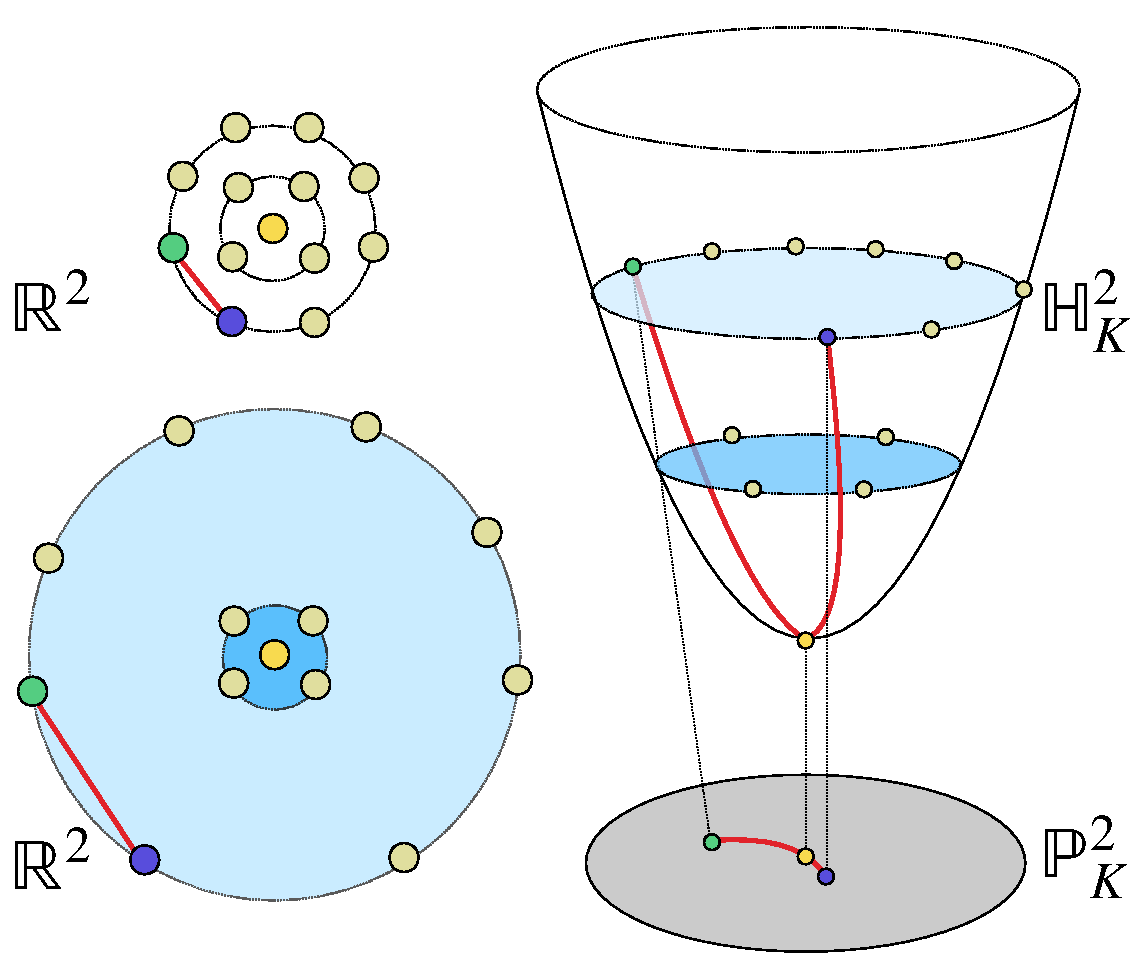
\includegraphics[width=0.9\linewidth]{explanatory_fig.pdf}
    \vspace{-10pt}
    \caption{The shortest path between a given pair of node embeddings in $\mathbb{R}^2$ and hyperbolic space as modelled by the Lorentz model $\mathbb{H}^2_K$ and Poincar\'e disk $\mathbb{P}^2_K$. Unlike Euclidean space, distances between points grow exponentially as you move away from the origin in hyperbolic space, and thus the shortest paths between points in hyperbolic space go through a common parent node, ---i.e. the origin, giving rise to hierarchical and tree-like structure. }
    \vspace{-10pt}
    \label{fig:explanatory_fig_1}
\end{figure}

However, current normalizing flows are restricted to Euclidean space, and as a result, these approaches are ill-equipped to model data with an underlying hierarchical structure. %and fail to incorporate structural inductive biases.
%As a result, the learning problem often needs to \textit{rediscover} structure---such as hierarchy---that is known {\em a priori}.
%While  they fail to incorporate known structure in data burdening the learning problem as it needs to \textit{rediscover} structure that is known apriori. 
Many real-world datasets, such as ontologies, social networks, sentences in natural language, and evolutionary relationships between biological entities in phylogenetics exhibit rich hierarchical or tree-like structure.
Hierarchical data of this kind can be naturally represented in hyperbolic spaces, \ie, non-Euclidean spaces with constant negative curvature (Figure \ref{fig:explanatory_fig_1}). 
But Euclidean normalizing flows fail to incorporate these structural inductive biases, since Euclidean space cannot embed deep hierarchies without suffering from high distortion \cite{sarkar2011low}. Furthermore, sampling from densities defined on Euclidean space will inevitability generate points that do not lie on the underlying hyperbolic space. 
%Intuitively, this occurs due to a fundamental geometric limitation of Euclidean spaces.
%Hierarchies (i.e, trees) generally grow exponentially as their depth increases, and the homogeneous structure of Euclidean space is unable to embed such exponential growth. 

%embed deep hierarchies
%The main challenge of probabilistic modeling of hierarchical data is that conventional Euclidean spaces are ill-equipped to embed deep hierarchies
%observational data to continuous latent variables without suffering from high distortion \cite{sarkar2011low}. 
%Intuitively, this occurs due to a fundamental geometric limitation of Euclidean spaces.
%Hierarchies (i.e, trees) generally grow exponentially as their depth increases, and the homogeneous structure of Euclidean space is unable to embed such exponential growth. 
%Indeed, if an underlying data distribution lies on a hyperbolic manifold, performing density estimation in Euclidean space 

%Recently, hyperbolic spaces have been proposed as an alternative to embedding hierarchical data due to their attractive geometric properties. 
%For example, hyperbolic spaces can be thought of as the continuous analogs of trees and can be used to embed trees with arbitrarily low distortion. 

\xhdr{Present work} 
To address this fundamental limitation, we present the first extension of normalizing flows to hyperbolic spaces. 
%Our work answer the question: how can we learn rich probability distributions over hyperbolic latent variables? 
%Currently, there are no existing approaches to extend normalizing flows to hyperbolic spaces
%Despite the known importance of leveraging hyperbolic spaces for modeling hierarchical data \cite{nickel2018learning}, there are no existing approaches for flexible density estimation on hyperbolic spaces. 
Prior works have considered learning models with hyperbolic parameters  \cite{liu2019hyperbolic,nickel2018learning} as well as variational inference with hyperbolic latent variables \cite{nagano2019wrapped,mathieu2019continuous}, but our work represents the first approach to allow flexible density estimation in hyperbolic space. 
%but the approximate posterior distribution is still limited due to the mean-field assumption. 
%In this work, we answer the following question: how can we learn rich probability distributions over hyperbolic latent variables? 
%using stochastic variational inference that better approximate true posteriors for hierarchical data?

%We appeal to the geometry of hyperbolic spaces and construct novel normalizing flows in the Lorentz model of hyperbolic geometry. 
To define our normalizing flows we leverage the Lorentz model of hyperbolic geometry and introduce two new forms of coupling, {\em Tangent Coupling} ($\mathcal{TC}$) and {\em Wrapped Hyperboloid Coupling} ($\mathcal{W}\mathbb{H}\mathcal{C}$). These define flexible and invertible transformations capable of transforming sampled points in the hyperbolic space. 
We derive the change of volume associated with these transformations and show that it can be computed efficiently with $\mathcal{O}(n)$ cost, where $n$ is the dimension of the hyperbolic space.
We empirically validate our proposed normalizing flows on structured density estimation, reconstruction and generation tasks on hierarchical data, highlighting the utility of our proposed approach. \cut{We find that using Wrapped Hyperbolic flows allows for a \red{\%XX} an aggregate absolute improvement over Euclidean flows.}


\section{Background on Hyperbolic Geometry}\label{sec:background}

Within Riemannian geometry, hyperbolic space is a manifold with constant negative curvature $K$ and is of particular interest for embedding hierarchical structures. There are multiple isometries of $n$-dimensional hyperbolic space, such as the hyperboloid $\mathbb{H}_K^n$, also known as the Lorentz model, or the Poincar\'e disk $\mathbb{D}_K^n$. Figure \ref{fig:explanatory_fig_1} illustrates some key properties of $\mathbb{H}_K^n$ and $\mathbb{D}_K^n$, highlighting how distances grow exponentially as you move away from the origin and how the shortest paths between points tend to go through the origin, giving rise to heirarchical or tree-like structure. %how a two-dimensional hyperbolic space can perfectly embed a tree with arbitrarily low distortion \cite{sarkar2011low}%, which is not possible in Euclidean spaces as it does not grow exponentially like the former leaving little room to place nodes. 
%Crucially, this implies that shortest distance between two given leaves, denoted by the red line, respects the hierarchical structure and must go pass through the origin (yellow node) in hyperbolic space but not in Euclidean space. 
In the next section we briefly review the Lorentz model of hyperbolic geometry. We are not assuming background in Riemannian geometry, though Appendix \ref{riemannian_geometry_appendix} and \citet{Ratcliffe94} are of use to the interested reader. Henceforth, for notational clarity, we use boldface font to denote points on the hyperboloid manifold.


% We briefly review the Lorentz model of hyperbolic geometry. We are not
% assuming background in Riemannian geometry (Appendix \ref{riemannian_geometry_appendix}); \cut{one can understand concepts
% like curvature intuitively without needing a long digression into
% Riemannian geometry.} a very useful source is \cite{Ratcliffe94}. Henceforth, for notational clarity, we use boldface font to denote points on the hyperboloid manifold.

\subsection{Lorentz Model of Hyperbolic Geometry}
%Historically, hyperbolic space arose as an example of a geometry that is internally consistent but breaks Euclid's parallel postulate.  
An $n-$dimensional hyperbolic space, $\mathbb{H}^n_K$, is the unique, complete, simply-connected $n-$dimensional Riemannian manifold of constant negative curvature, $K$.  For our purposes the Lorentz model is the most convenient representation of hyperbolic space, since it is equipped with relatively simple explicit formulas and useful numerical stability properties \cite{nickel2018learning}. The Lorentz model embeds hyperbolic space $\mathbb{H}^n_K$ within the $n+1-$dimensional Minkowski space, defined as the manifold $\mathbb{R}^{n+1}$ equipped with the following inner product:
\begin{equation}\label{eq:lorentzmetric}
    \langle \textbf{x}, \textbf{y} \rangle_{\mathcal{L}} := -x_0y_0 + x_1y_1 + \dots + x_ny_n,
\end{equation}
which has the type 
$\langle \cdot, \cdot \rangle_{\mathcal{L}}: \mathbb{R}^{n+1} \times \mathbb{R}^{n+1} \to \mathbb{R}$.
%It is indefinite, which may come as a shock to those used to the traditional definition of inner product from linear algebra, but this is a well-defined notion extensively used in special relativity for over a century.  
It is common to denote this space as $\mathbb{R}^{1,n}$ to emphasize the distinct role of the zeroth coordinate.
In the Lorentz model, we model hyperbolic space as the (upper sheet of) the hyperboloid embedded in Minkowski space. It is a remarkable fact that though the Lorentzian metric (Eq.~\ref{eq:lorentzmetric}) is indefinite,
the induced Riemannian metric $g_{\mb{x}}$ on the unit hyperboloid is positive definite \cite{Ratcliffe94}. The $n-$Hyperbolic space with constant negative curvature $K$ with origin $\textbf{o} = (1/K, 0, \dots, 0)$, is a Riemannian manifold $(\mathbb{H}^{n}_K,g_{\mb{x}})$ where
\begin{equation*}
    \mathbb{H}^{n}_K := \{x \in \mathbb{R}^{n+1}:  \langle \textbf{x}, \textbf{x} \rangle_{\mathcal{L}} = 1/K, \ x_0 > 0, \ K<0 \},
\end{equation*}

%If we define $d_{\mathbb{H}^{n}_K} = $
%Indeed, if we define $d_{\mathbb{H}^{n}_K}(\mathbf{x},\mathbf{y})$ by $\langle \textbf{x},\textbf{y} \rangle_{\mathcal{L}}  = ||\bx||||\by||\cosh d_{\mathbb{H}^{n}_K}(\bx,\by)$ then $d_{\mathbb{H}^{n}_K}$ is a metric on the hyperbolic space \cite{Ratcliffe94}.
%; see~\cite{Ratcliffe94} page 64.
%Describing hyperbolic space in this way is convenient as one can use the coordinates in the embedding space to write explicit formulas for derivatives and other operations.  
%When convenient we shall also use the generalized radius $R = 1/\sqrt{-K}$ in place of the curvature.

Equipped with this, the induced distance between two points $(\mb{x},\mb{y})$ in $\mathbb{H}^{n}_K$ is given by
\begin{equation}
    d(\textbf{x},\textbf{y})_{\mathcal{L}} := \frac{1}{\sqrt{-K}}\arccosh(-K \langle \textbf{x}, \textbf{y} \rangle_{\mathcal{L}}).
\end{equation}
%This is obtained by inverting the relation for $\eta$ described above.

The tangent space to the hyperboloid at the point $\textbf{p} \in \mathbb{H}_K^n$ can also be described as an embedded subspace of $\mathbb{R}^{1,n}$.  
It is given by the set of points satisfying the orthogonality relation with respect to the Minkowski inner product \footnote{It is also equivalently known as the Lorentz inner product.},
\begin{equation}
    \mathcal{T}_{\textbf{p}}\mathbb{H}^n_K := \{u: \langle u, \textbf{p} \rangle_{\mathcal{L}} = 0 \}.
\end{equation}
Of special interest are vectors in the tangent space at the origin of $\mathbb{H}^{n}_K$ whose norm under the Minkowski inner product is equivalent to the conventional Euclidean norm. That is $v \in \mathcal{T}_{\textbf{o}}\mathbb{H}^{n}_K$ is a vector such that $v_0 = 0$ and $||\textbf{v}||_{\mathcal{L}} := \sqrt{\langle \textbf{v}, \textbf{v}
\rangle_{\mathcal{L}}} = ||\textbf{v}||_2$.  Thus \emph{at the origin} the
partial derivatives with respect to the ambient coordinates, $\mathbb{R}^{n+1}$, defines the
covariant derivative.  
%Of course, this is not generally true at other points but we will define our transformations such that we only require derivatives at the origin.

\xhdr{Projections}
Starting from the extrinsic view by which we consider $\mathbb{R}^{n+1} \supset \mathbb{H}^{n}_K$, we may project any vector $x \in \mathbb{R}^{n+1}$ on to the hyperboloid using the shortest Euclidean distance:
\begin{equation}
    \textnormal{proj}_{\mathbb{H}^{n}_K}(x) = \frac{x}{\sqrt{-K}||x||_{\mathcal{L}}}.
\end{equation}
Furthermore, by definition a point on the hyperboloid satisfies $\langle \textbf{x}, \textbf{x} \rangle_{\mathcal{L}} = 1/K$ and thus when provided with $n$ coordinates $\hat{x} = (x_1, \dots, x_{n})$ we can always determine the missing coordinate to get a point on $\mathbb{H}^n_K$:
\begin{equation}
    \label{eqn:hyperboloid_projection}
    x_0 = \sqrt{||\hat{x}||^2_2 + \frac{1}{K}}.
\end{equation}
%We later exploit this fact in \ref{wrapped_hyerboloid_coupling_section}, to determine points on $\mathbb{H}^n_K$ that our normalizing flow should transport to.

\xhdr{Exponential Map}
The exponential map takes a vector, $v$, in the tangent space of a point $\textbf{x} \in \mathbb{H}^{n}_K$ to a point on the manifold---i.e., $\textbf{y} = \textnormal{exp}^K_\textbf{x}(v): \mathcal{T}_{\textbf{x}} \mathbb{H}^{n}_K \to \mathbb{H}^{n}_K$ by moving a unit length along the \textit{geodesic}, $\gamma$ (straightest parametric curve), uniquely defined by $\gamma(0) = \textbf{x}$ with direction $\gamma '(0)= v$. The closed form expression for the Lorentz model is then given by
\begin{equation}
    \label{eqn:exp_map}
    \textnormal{exp}^K_{\textbf{x}} (v) = \cosh \Big(\frac{||v||_{\mathcal{L}}}{R} \Big)\textbf{x} +  \sinh \Big(\frac{||v||_{\mathcal{L}}}{R} \Big)\frac{Rv}{||{v}||_{\mathcal{L}}},
\end{equation}
where we used the \textit{generalized radius} $R = 1/\sqrt{-K}$ in place of the curvature.

\xhdr{Logarithmic Map}
As the inverse of the exponential map, the logarithmic map takes a point, $\textbf{y}$, on the manifold back to the tangent space of another point $\textbf{x}$ also on the manifold. In the Lorentz model this is defined as
\begin{equation}
    \label{eqn:log_map}
    \log^K_{\textbf{x}}{\textbf{y}} = \frac{\arccosh(\alpha)}{\sqrt{\alpha^2 - 1}}(\textbf{y} - \alpha \textbf{x}),
\end{equation}
where $\alpha = K\langle \textbf{x}, \textbf{y} \rangle_{\mathcal{L}}$.

\xhdr{Parallel Transport}
The parallel transport for two points $\textbf{x},\textbf{y} \in \mathbb{H}^{n}_K$ is a map that carries the vectors in $v \in \mathcal{T}_{\textbf{x}}\mathbb{H}^{n}_K$ to corresponding vectors at $v' \in \mathcal{T}_{\textbf{y}}\mathbb{H}^{n}_K$ along the geodesic. That is vectors are connected between the two tangent spaces such that the covariant derivative is unchanged. For Riemannian Manifolds we use the Levi-Civita connection. Parallel transport is a map that preserves the metric tensor, \ie, $\langle \textnormal{PT}^K_{\textbf{x} \to \textbf{y}}(v), \textnormal{PT}^K_{\textbf{x} \to \textbf{y}}(v') \rangle_{\mathcal{L}} = \langle v, v' \rangle_{\mathcal{L}}$ and in the Lorentz model is given by
\begin{align}
    \label{eqn:parallel_transport}
    \textnormal{PT}^K_{\textbf{x} \to \textbf{y}}(v) & = v - \frac{ \langle \log^K_{\textbf{x}}(\textbf{y}), v \rangle_{\mathcal{L}}}{d(\textbf{x},\textbf{y})_{\mathcal{L}}} (\log^K_{\textbf{x}}(\textbf{y})+ \log^K_{\textbf{y}}(\textbf{x})) \nonumber \\
    & = v + \frac{ \langle \textbf{y}, v \rangle_{\mathcal{L}}}{R^2 - \langle \textbf{x}, \textbf{y} \rangle_{\mathcal{L}}} (\textbf{x}+ \textbf{y}),
\end{align}
where $\alpha$ is as defined above. Another useful property is that the inverse parallel transport simply carries the vectors back along the geodesic and is simply defined as $(\textnormal{PT}^{K}_{\textbf{x} \to \textbf{y}}(v))^{-1} = \textnormal{PT}^K_{\textbf{y} \to \textbf{x}}(v)$.

\subsection{Probability Distributions on Hyperbolic Spaces}\label{sec:hyperprobs}

Probability distributions can be defined on Riemannian manifolds which includes $\mathbb{H}^n_K$ as a special case, by relating an infinitesimal volume on the manifold to a corresponding volume in a homeomorphic Euclidean space by the conservation of measure.
In particular, given the Riemannian manifold $\mathcal{M}(\textbf{z})$ and its metric $g_\mb{z}$, we have $\int p(\textbf{z}) d\mathcal{M} (\textbf{z}) = \int p(\textbf{z})\sqrt{|g_\mb{z}|}d \textbf{z}$, where $d \textbf{z}$ is the Lebesgue measure. We now briefly survey three distinct generalizations of the normal distribution to Riemannian manifolds.\cut{ following ~\cite{mathieu2019continuous,skopek2019mixed}.}

\xhdr{Riemannian Normal}
The first is the Riemannian normal~\cite{pennec2006intrinsic, said2014new}, which is derived from maximizing the entropy given a mean $\mu$ and a variance $\sigma$.
Specifically, we have $\mathcal{N}_{\mathcal{M}}(\textbf{z} \vert \mu, \sigma^{2}) = \frac{1}{Z} \exp \left( - d_{\mathcal{M}}(\mu, \textbf{z})^2 / 2 \sigma^{2} \right)$, where $d_{\mathcal{M}}$ is the \textit{induced distance} and $Z$ is the normalization constant \cite{said2014new, mathieu2019continuous}.

\xhdr{Restricted Normal}
One can also restrict sampled points from the normal distribution in the ambient space to the manifold.
One example is the Von Mises distribution on the unit circle and its generalized version, \ie, Von Mises-Fisher distribution on the hypersphere~\cite{davidson2018hyperspherical}.

\xhdr{Wrapped Normal}
Finally, we can define a wrapped normal distribution~\cite{falorsi2019reparameterizing,nagano2019wrapped}, which is obtained by (1) sampling from $\mathcal{N}(0,I)$ and then transforming it to a point $v \in \mathcal{T}_\textbf{o}\mathbb{H}_K^n$ by concatenating $0$ as the zeroth coordinate; (2) parallel transporting the sample $v$ from the tangent space at $\textbf{o}$ to the tangent space of another point $\boldsymbol{\mu} $ on the manifold to obtain $u$; (3) mapping $u$ from the tangent space to the manifold using the exponential map at $\boldsymbol{\mu}$.
Sampling from such a distribution is straightforward and the probability density can be obtained via the change of variable formula,
\begin{align}
    \log p(\textbf{z}) = \log p(v) - (n-1) \log \left(\frac{\sinh{ ( \Vert u \Vert_{\mathcal{L}} ) }}{ \Vert u \Vert_{\mathcal{L}} } \right),
\end{align}
where $p(\textbf{z})$ is the wrapped normal distribution and $p(v)$ is the normal distribution in the tangent space of $\textbf{o}$.





\section{Normalizing Flows on Hyperbolic Spaces}
We seek to define flexible and learnable distributions on $\mathbb{H}^n_K$, which will allow us to learn rich approximate posterior distributions for hierarchical data.
To do so, we design a class of invertible parametric hyperbolic functions, $f_i: \mathbb{H}^n_K \to \mathbb{H}^n_K$.
A sample from the approximate posterior can then be obtained by first sampling from a simple base distribution $\mb{z}_0 \sim p(\mb{z})$ defined on $\mathbb{H}^n_K$ and then applying a composition of  functions $f_{i\in[j]}$ from this class: $\mb{z}_j = f_j \circ f_{j-1} \circ \dots \circ f_1(\mb{z}_0)$.

In order to ensure effective and tractable learning, the class of functions $f_i$ must satisfy three key desiderata:
\begin{enumerate}[itemsep=0pt, parsep=0pt, topsep=0pt]
    \item Each function $f_i$ must be invertible. 
    \item We must be able to efficiently sample from the final distribution, $\mb{z}_j = f_j \circ f_{j-1} \circ \dots \circ f_1(\mb{z}_0)$. 
    \item We must be able to efficiently compute the associated change in volume ---i.e., the Jacobian determinant, of the overall transformation.
\end{enumerate}
 Given these requirements, the final transformed distribution is given by the change of variables formula:
\begin{equation}
    \log p(\mb{z}_j) = \log p(\mb{z}_0) - \sum_{i=1}^k\log \textnormal{det}\Big|\frac{\partial f_j}{\partial z_{j-1}} \Big|.
    \vspace{-5pt}
\end{equation}

Functions satisfying desiderata 1-3 in Euclidean space are often termed {\em normalizing flows} (Appendix \ref{normalizing_flow_appendix}), and our work extends this idea to hyperbolic spaces. In the following sections, we describe two flows of increasing complexity, Tangent Coupling ($\mathcal{T}C$) and Wrapped Hyperboloid Coupling ($\mathcal{W}HC$). The first approach lifts a standard Euclidean flow to the tangent space at the origin of the hyperboloid.
The second approach modifies the flow to explicitly utilize hyperbolic geometry. Figure \ref{fig:density_estimation} illustrates synthetic densities as learned by our approach on $\mathbb{P}^2_1$. 

\subsection{Tangent Coupling}
Similar to the Wrapped Normal distribution (Section \ref{sec:hyperprobs}), one strategy to define a normalizing flow on the hyperboloid is to use the tangent space at the origin. That is, we first sample a point from our base distribution---which we define to be a Wrapped Normal---and use the logarithmic map at the origin to transport it to the corresponding tangent space. Once we arrive at the tangent space we are free to apply any Euclidean flow before finally projecting back to the manifold using the exponential map. 
This approach leverages the fact that the tangent bundle of a hyperbolic manifold has a well-defined vector space structure, allowing affine transformations and other operations that are ill-defined on the manifold itself. 
%the disjoint union of all tangent spaces, \textit{tangent bundle}, of a hyperbolic manifold has a well-defined vector space structure, allowing affine transformations and other operations that are ill-defined on the manifold itself. 

Following this idea, we build upon one of the earliest and most well-studied flows: the RealNVP flow \cite{dinh2016density}. At its core, the RealNVP flow uses a computationally symmetric transformation (affine coupling layer) which has the benefit of being fast to evaluate and invert due to its lower triangular Jacobian, whose determinant is cheap to compute. Operationally, the coupling layer is implemented using a binary mask, and partitions some input $\tilde{x}$ into two sets, where the first set, $\tilde{x}_1:=\tilde{x}_{1:d}$ is transformed elementwise independently of other dimensions. The second set, $\tilde{x}_2:=\tilde{x}_{d+1:n}$, is also transformed elementwise but in a way that depends on the first set (see Appendix \ref{Euclidean_RealNVP_appendix} for more details). Since all coupling layer operations occur at $\mathcal{T}_{\textbf{o}}\mathbb{H}^n_K$ we term this form of coupling as Tangent Coupling ($\mathcal{T}C$). 

Thus the overall transformation due to one layer of our $\mathcal{T}C$ flow is a composition of a logarithmic map, affine coupling defined on $\mathcal{T}_{\textbf{o}}\mathbb{H}^n_k$, and an exponential map:
\begin{align}
    \label{eq:tangent_coupling}
     \tilde{f}^{\mathcal{T}C}(\tilde{x}) &=
     \begin{cases}
     \tilde{z}_{1} &= \tilde{x}_{1} \\
     \tilde{z}_{2} &= \tilde{x}_{2} \odot \sigma(s(\tilde{x}_{1})) + t(\tilde{x_1}) \nonumber
     \end{cases}\\
    %f(\tilde{x}) &=  b \odot \tilde{x} + (1 - b)\odot(\tilde{x} \odot \sigma(s(b \odot \tilde{x})) + t(b \odot \tilde{x})) \nonumber \\
    %\textbf{y} =&  \textnormal{exp}_{\textbf{o}}(f(\tilde{x})) ,
    f^{\mathcal{T}C}(\mb{x}) &= \textnormal{exp}_{\textbf{o}}^K(\tilde{f}^{\mathcal{T}C}(\log_{\textbf{o}}^K(\textbf{x}))),
\end{align}

where $\tilde{x} = \log_{\textbf{o}}^K(\textbf{x})$ is a point on $\mathcal{T}_{\textbf{o}}\mathbb{H}^n_K$, and $\sigma$ is a pointwise non-linearity such as the exponential function. Functions $s$ and $t$ are parameterized scale and translation functions implemented as neural nets from $\mathcal{T}_{\textbf{o}}\mathbb{H}^{d}_K \to \mathcal{T}_{\textbf{o}}\mathbb{H}^{n-d}_K$.
One important detail is that arbitrary operations on a tangent vector $v \in \mathcal{T}_{\textbf{o}}\mathbb{H}^n_K$ may transport the resultant vector outside the tangent space, hampering subsequent operations.
To avoid this we can keep the first dimension fixed at $v_0 = 0$ to ensure we remain in $\mathcal{T}_{\textbf{o}}\mathbb{H}^{n}_K$.

\begin{figure}[t!]
     \centering
     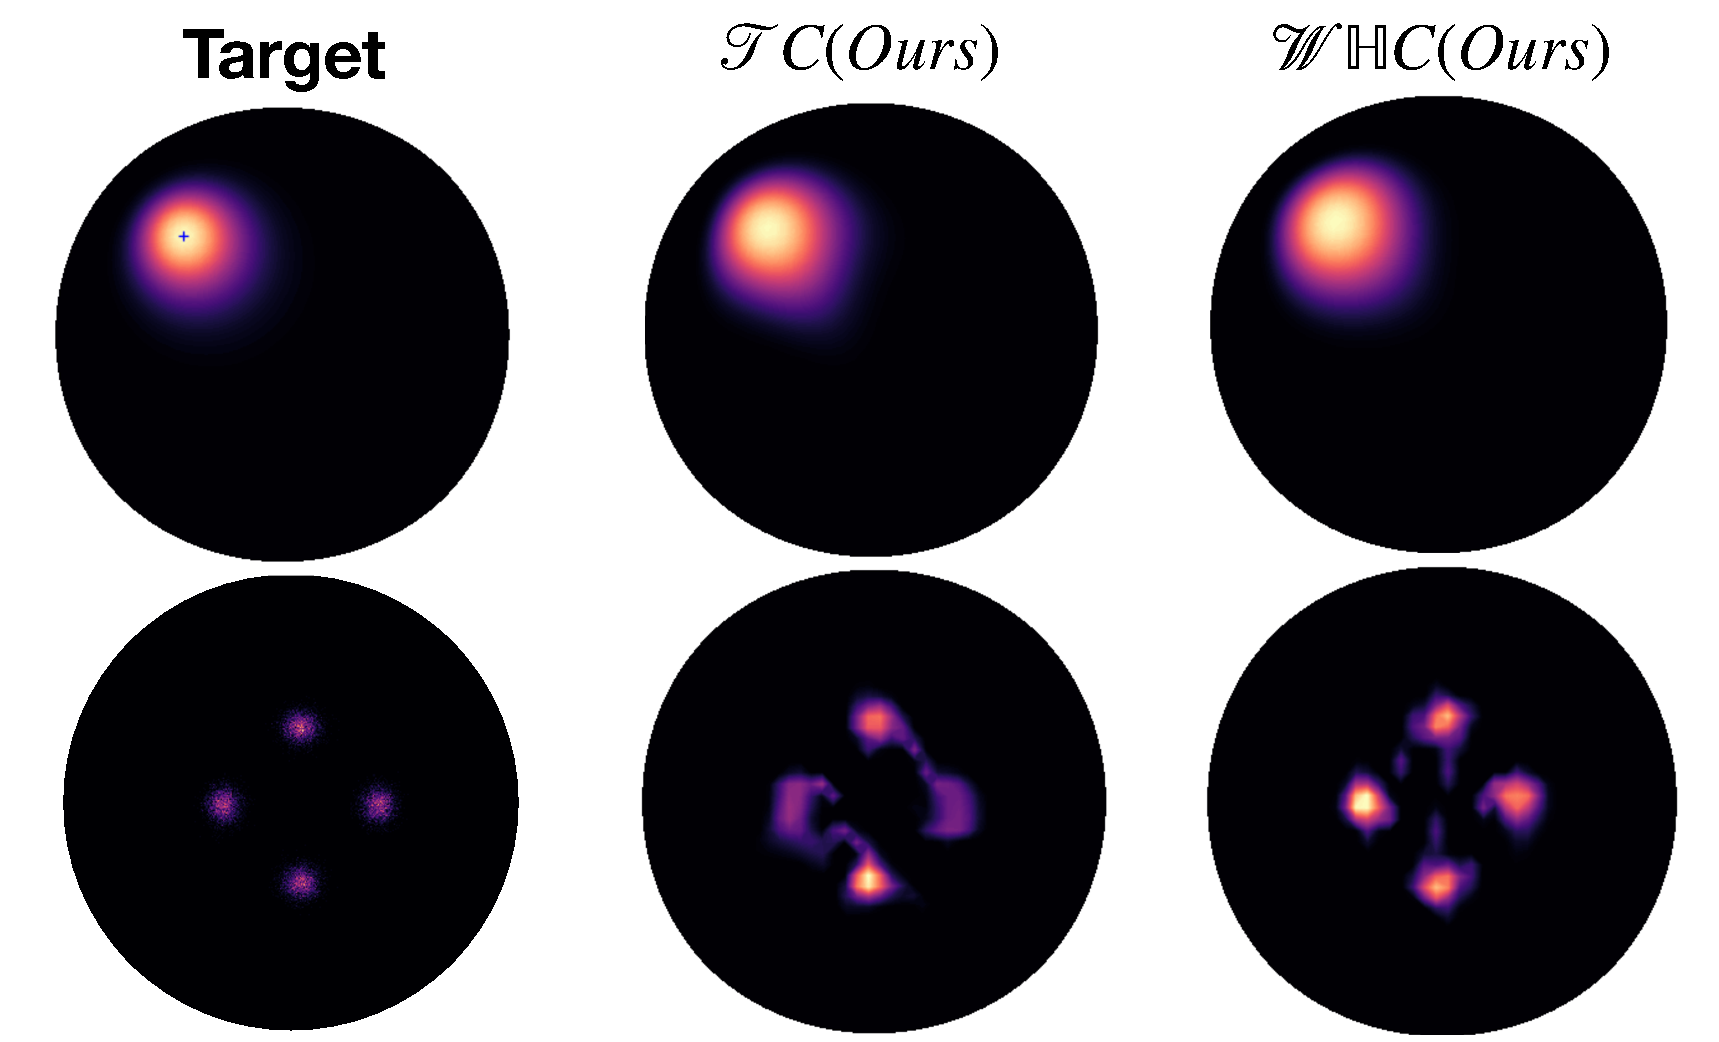
\includegraphics[width=0.95\linewidth]{hyperbolic_density_graphic.pdf}
     \vspace{-10pt}
     \caption{Comparison of density estimation in hyperbolic space for 2D wrapped Gaussian (WG) and mixture of wrapped gaussian (MWG) on $\mathbb{P}^2_1$. Densities are visualized in the Poincar\'e disk.}
     \vspace{-10pt}
     \label{fig:density_estimation}
 \end{figure}

Similar to the Euclidean RealNVP, we need an efficient expression for the Jacobian determinant of $f^{\mathcal{T}C}$.
\begin{prop}
The Jacobian determinant of a single $\mathcal{T}C$ layer in \eqref{eq:tangent_coupling} is:
\begin{align}
     \left|\textnormal{det}\Big (\frac{\partial \textbf{y}}{\partial \textbf{x}}\Big)\right| &= \Big(\frac{R\sinh(\frac{||z||_{\mathcal{L}}}{R})}{||z||_{\mathcal{L}}}\Big)^{n-1} \times \prod_{i=d+1}^n\sigma(s(\tilde{x}_1))_i  \nonumber\\
     & \times \Big(\frac{R\sinh(\frac{||\log^K_{\textbf{o}}(\textbf{x})||_{\mathcal{L}}}{R})}{||\log^K_{\textbf{o}}(\textbf{x})||_{\mathcal{L}}}\Big)^{1-n}
    %\label{jac_det_tangent_flow_1}.
\end{align}
where, $ \mb{z} =  \tilde{f}^{\mathcal{T}C}(\tilde{x})$ and $\tilde{f}^{\mathcal{T}C}$ is as defined above.
\end{prop}
\begin{proofsketch}
Here we only provide a sketch of the proof and details can be found in Appendix \ref{tangent_coupling_proof_appendix}. First, observe  that the overall transformation  is a valid composition of functions: $\mb{y} := \textnormal{exp}_{\textbf{o}}^K \circ \tilde{f}^{\mathcal{T}C} \circ \log_{\textbf{o}}^K(\textbf{x})$. Thus, the overall determinant can be computed by chain rule and the identity,  $\textnormal{det}\Big (\frac{\partial \textbf{y}}{\partial \textbf{x}}\Big) =  \textnormal{det}\Big (\frac{\partial \textnormal{exp}_{\textbf{o}}^K(z)}{\partial z}\Big) \cdot \textnormal{det}\Big (\frac{\partial f(\tilde{x})}{\partial \tilde{x}}\Big) \cdot  \textnormal{det}\Big (\frac{\partial \log_{\textbf{o}}^K(\textbf{x})}{\partial \textbf{x}}\Big)$. Tackling each function in the composition individually, $\textnormal{det}\Big (\frac{\partial \textnormal{exp}_{\textbf{o}}^K(z)}{\partial z}\Big) = \Big(\frac{R\sinh(\frac{||z||_{\mathcal{L}}}{R})}{||z||_{\mathcal{L}}}\Big)^{n-1}$ as derived in \citet{skopek2019mixed}. As the logarithmic map is the inverse of the exponential map the Jacobian determinant is simply the inverse of the determinant of the exponential map, which gives the $\textnormal{det}\Big (\frac{\partial \log_{\textbf{o}}^K(\textbf{x})}{\partial \textbf{x}}\Big)$ term. 
For the middle term, we must calculate the directional derivative of $\tilde{f}^{\mathcal{T}C}$ in an orthonormal basis w.r.t. the Lorentz inner product, of $\mathcal{T}_{\textbf{o}}\mathbb{H}^{n}_K$. Since the standard Euclidean basis vectors $e_1, ..., e_n$ are also a basis for $\mathcal{T}_{\textbf{o}}\mathbb{H}^{n}_K$, the Jacobian determinant $\textnormal{det}\Big (\frac{\partial f(\tilde{x})}{\partial \tilde{x}}\Big)$ simplifies to that of the RealNVP flow, which is lower triangluar and is thus efficiently computable in $\mathcal{O}(n)$ time.

\end{proofsketch}
It is remarkable that the middle term in Proposition 1 is precisely the same change in volume associated with affine coupling in RealNVP.
The change in volume due to the hyperbolic space only manifests itself through the exponential and logarithmic maps, each of which can be computed in $\mathcal{O}(n)$ cost. Thus, the overall cost is only slightly larger than the regular Euclidean RealNVP, but still $\mathcal{O}(n)$.

\subsection{Wrapped Hyperboloid Coupling}
\begin{figure}[ht]
    \centering
    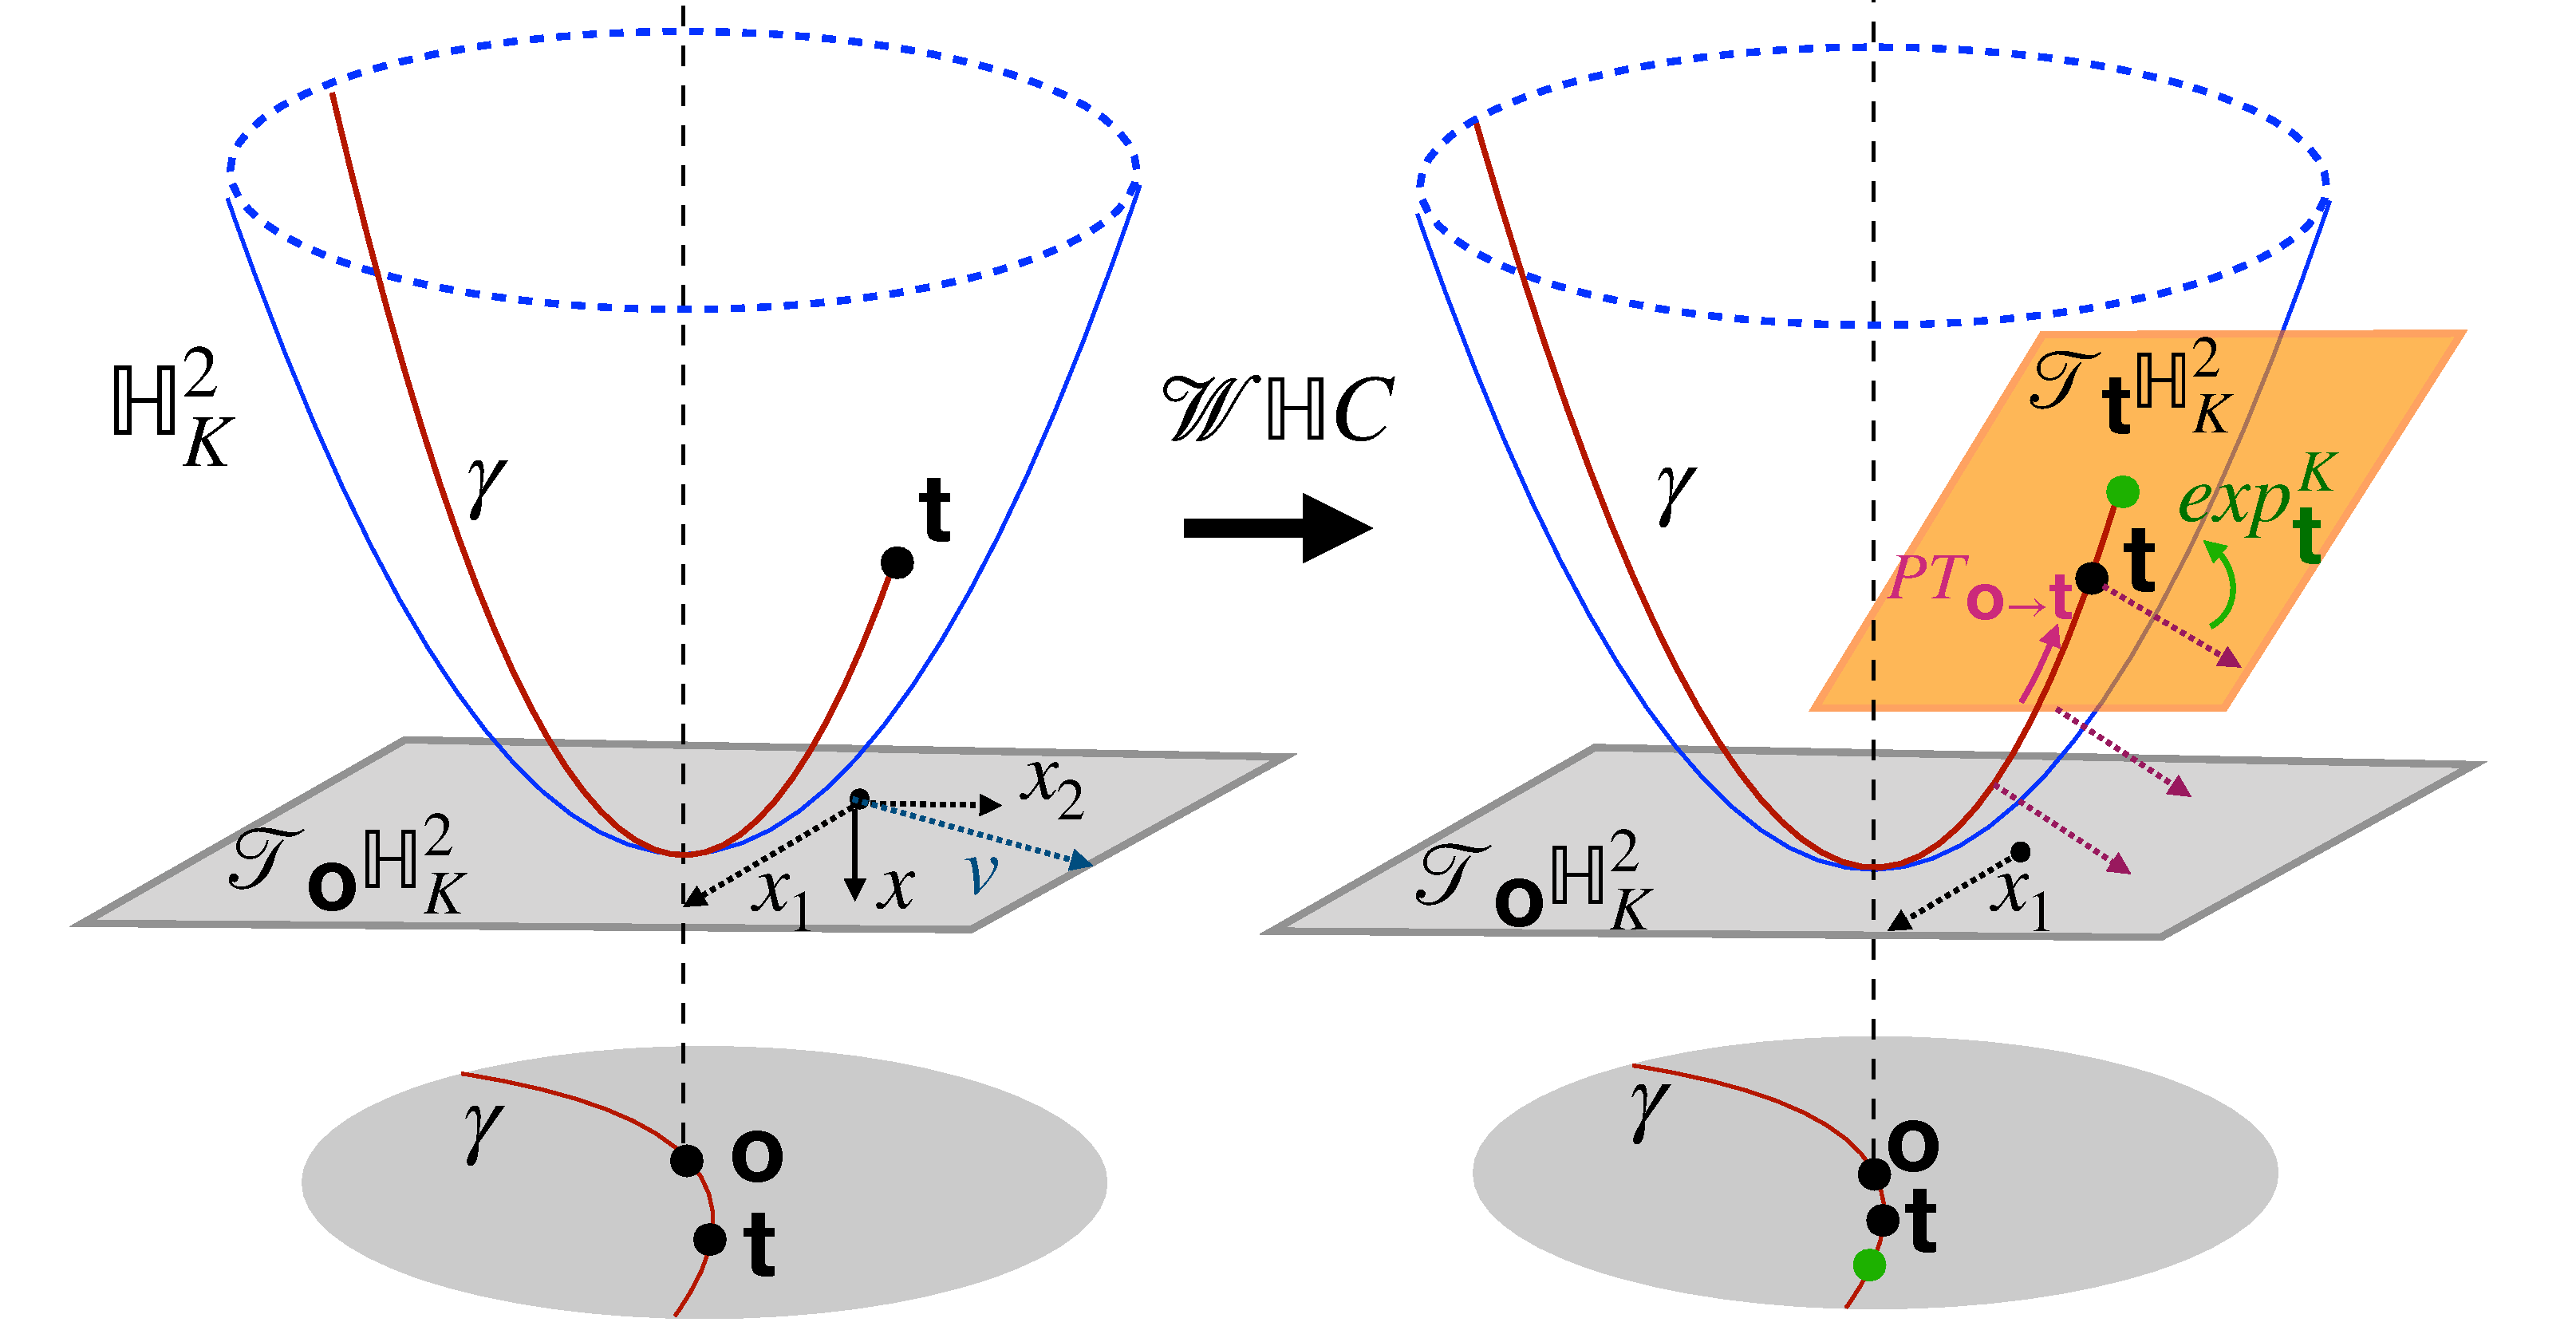
\includegraphics[width=0.95\linewidth]{hyperbolic_flows_arch.pdf}
    %\vspace{-5mm}
    \caption{Wrapped Hyperbolic Coupling. The left figure depicts a partitioned input point $\tilde{x}_1:=\tilde{x}_{1:d}$ and $\tilde{x}_2:=\tilde{x}_{d+1:n}$ prior to parallel transport. The right figure depicts the $\tilde{x}_2$ vector after it is transformed, parallel transported, and projected to $\mathbb{H}^n_K$.}
    %\vspace{-5pt}
    \label{fig:whc_architecture_diagram}
\end{figure}

\label{wrapped_hyerboloid_coupling_section}
The hyperbolic normalizing flow with $\mathcal{T}C$ layers discussed above operates purely in the tangent space at the origin.
This simplifies the computation of the Jacobian determinant, but anchoring the flow at the origin may hinder its expressive power and its ability to leverage disparate regions of the manifold. 
In this section, we remedy this shortcoming with a new hyperbolic flow that performs translations between tangent spaces via parallel transport. 
%which may lack expressive power. That is to say, by utilizing solely the tangent space at the origin the normalizing flow doesn't utilize different regions of the manifold which may be useful to learning richer and more flexible distributions. One remedy to this fact is to make more explicit use of the manifold by defining different flow operations on different tangent spaces. Specifically, we can define the translation function, $t$, as predicting a tangent space we wish to Parallel transport to rather than simply translating a vector in $\mathcal{T}_{\textbf{o}}\mathbb{H}^n_K$.

We term this transformation {\em Wrapped Hyperboloid Coupling} ($\mathcal{W}\mathbb{H}C$). %which we compose to define a new normalizing flow.
As with the $\mathcal{T}C$ layer, it is a fully invertible transformation $f^{\mathcal{W}\mathbb{H}C}: \mathbb{H}^n_k \to \mathbb{H}^n_k$ with a tractable analytic form for the Jacobian determinant. 
%that learns to transport different partitions of the latent code to different points on the manifold. Critically, the associated change in volume due to $\mathcal{W}\mathbb{H}$-Coupling can be efficiently computed as the Jacobian determinant retains a block triangular structure. 
To define a $\mathcal{W}\mathbb{H}C$ layer we first use the logarithmic map at the origin to transport a point to the tangent space. We employ the coupling strategy previously discussed and partition our input vector into two components: $\tilde{x}_1:=\tilde{x}_{1:d}$ and $\tilde{x}_2:=\tilde{x}_{d+1:n}$. Let $\tilde{x} = \log_{\textbf{o}}^K(\mb{x})$ be the point on $\mathcal{T}_{\textbf{o}}\mathbb{H}^n_K$ after the logarithmic map. 
The remainder of the $\mathcal{W}\mathbb{H}C$ layer can be defined as follows;
\begin{align}
\label{wrapped_hyperboloid_coupling_eqn}
\tilde{f}^{\mathcal{W}\mathbb{H}C}(\tilde{x})&=
     \begin{cases}
     \tilde{z}_{1} &= \tilde{x}_{1}  \\
     \tilde{z}_{2} &= \log_{\textbf{o}}^K\Big( \textnormal{exp}_{t(\tilde{x}_{1})}^K\big(\textnormal{PT}_{\textbf{o}\to t(\tilde{x}_{1}) }(v)\big)\Big) \nonumber
    \end{cases}\\
    v &= \tilde{x}_{2} \odot \sigma(s(\tilde{x}_{1})) \nonumber \\
    f^{\mathcal{W}\mathbb{H}C}(\mb{x}) &=  \textnormal{exp}_{\textbf{o}}^K(\tilde{f}^{\mathcal{W}\mathbb{H}C}(\log_{\textbf{o}}^K(\mb{x}))).
\end{align}

Functions $s: \mathcal{T}_{\textbf{o}}\mathbb{H}^{d}_k \to \mathcal{T}_{\textbf{o}}\mathbb{H}^{n-d}_k$ and $t:\mathcal{T}_{\textbf{o}}\mathbb{H}^{d}_k \to \mathbb{H}^n_k$ are taken to be arbitrary neural nets, but the role of $t$ when compared to $\mathcal{T}C$ is vastly different. In particular, the generalization of translation on Riemannian manifolds can be viewed as parallel transport to a different tangent space. Consequently, in Eq.~\ref{wrapped_hyperboloid_coupling_eqn}, the function $t$ predicts a point on the manifold that we wish to parallel transport to.
This greatly increases the flexibility as we are no longer confined to the tangent space at the origin. The logarithmic map is then used to ensure that both $\tilde{z}_1$ and $\tilde{z}_2$ are in the same tangent space before the final exponential map that projects the point to the manifold.

One important consideration in the construction of $t$ is that it should only parallel transport functions of $\tilde{x}_2$. However, the output of $t$ is a point on $\mathbb{H}^n_k$ and without care this can involve elements in $\tilde{x}_1$. To prevent such a scenario we construct the output of $t = [t_0, 0, \dots , 0, t_{d+1}, \dots , t_{n}]$ where elements $t_{d+1:n}$ are used to determine the value of $t_0$ using Eq. \ref{eqn:hyperboloid_projection}, such that it is a point on the manifold and every remaining index is set to zero. Such a construction ensures that only components of any function of $\tilde{x}_2$ are parallel transported as desired. Figure \ref{fig:whc_architecture_diagram} illustrates the transformation performed by the $\mathcal{W}HC$ layer.

\xhdr{Inverse of $\mathcal{W}\mathbb{H}C$}
To invert the flow it is sufficient to show that argument to the final exponential map at the origin itself is invertible. Furthermore, note that $\tilde{x}_1$ undergoes an identity mapping and is trivially invertible. Thus we need to show that the second partition is invertible, i.e. that the following transformation is invertible:
\begin{equation}
     \tilde{z}_{2} = \log_{\textbf{o}}^K\Big( \textnormal{exp}_{t(\tilde{x}_{1})}^K\big(\textnormal{PT}_{\textbf{o}\to t(\tilde{x}_{1}) }(v)\big)\Big).
\end{equation}
As discussed in Section \ref{sec:background}, the parallel transport, exponential map, and logarithmic map all have well-defined inverses with closed forms. Thus, the overall transformation is invertible in closed form:
%By equation \ref{eqn:inv_parallel_transport} the inverse of parallel transport is another parallel transport. Also, by definition and equations \ref{eqn:exp_map}-\ref{eqn:log_map} the exponential and logarithmic maps are inverse mappings of each other. Consequently, the overall transformation is invertible and the closed form expression of the inverse is,
\begin{align*}
     \begin{cases}
     \tilde{x}_{1} &= \tilde{z}_{1} \\
     \tilde{x}_{2} &= \Big( \textnormal{PT}_{t(\tilde{z}_{1}) \to \textbf{o} }(\log_{t(\tilde{z}_{1})}^K( \textnormal{exp}_{\textbf{o}}^K(\tilde{z}_{2}))\Big) \odot \sigma(s(\tilde{z}_{1}))^{-1} \\
    \end{cases}
\end{align*}

\xhdr{Properties of $\mathcal{W}\mathbb{H}C$}
To compute the Jacobian determinant of the full transformation in Eq. \ref{wrapped_hyperboloid_coupling_eqn} we proceed by analyzing the effect of $\mathcal{W}\mathbb{H}C$ on valid orthonormal bases w.r.t. the Lorentz inner product for the tangent space at the origin. We state our main result here and provide a sketch of the proof, while the entire proof can be found in Appendix \ref{wrapped_coupling_proof_appendix}. 
\begin{prop}
The Jacobian determinant of the function $\tilde{f}^{\mathcal{W}\mathbb{H}C}$ in \eqref{wrapped_hyperboloid_coupling_eqn} is:
\begin{multline}
  \left|\textnormal{det}\left(\frac{\partial\mb{y}}{\partial \mb{x}}\right)\right| = \prod_{i=d+1}^n\sigma(s(\tilde{x}_1))_i \times \Big(\frac{R \sinh(\frac{||q||_{\mathcal{L}}}{R})}{||q||_{\mathcal{L}}}\Big)^{l} \\
  \times \Big(\frac{R\sinh(\frac{||\log_{\textbf{o}}^K(\hat{\textbf{q}})||_{\mathcal{L}}}{R})}{||\log_{\textbf{o}}^K(q)||_{\mathcal{L}}}\Big)^{-l} \ \times  \Big(\frac{R\sinh(\frac{||\tilde{z}||_{\mathcal{L}}}{R})}{||\tilde{z}||_{\mathcal{L}}}\Big)^{n-1}
 \  \\ \times \Big(\frac{R\sinh(\frac{||\log_{\textbf{o}}^K(\textbf{x})||_{\mathcal{L}}}{R})}{||\log_{\textbf{o}}^K(\textbf{x})||_{\mathcal{L}}}\Big)^{1-n},
\end{multline}
where $\tilde{z} = \textnormal{concat}(\tilde{z}_1, \tilde{z}_2)$, the constant $l = n-d$, $\sigma$ is a non-linearity, $q = \textnormal{PT}_{\textbf{o}\to t(\tilde{x}_1) }(v)$ and $\hat{\textbf{q}} = \textnormal{exp}_{\textbf{t}}^K(q)$.
\end{prop}
\begin{proofsketch}
We first note that the exponential and logarithmic maps applied at the beginning and end of the $\mathcal{W}\mathbb{H}C$ can be dealt with by appealing to the chain rule and the known Jacobian determinants for these functions as used in Proposition 1.  
Thus, what remains is the following term: $\left|\textrm{det}\left(\frac{\partial z}{\partial \tilde{x}}\right)\right|$. To evaluate this term we rely on the following Lemma.
\begin{lemma}
Let $h : \mc{T}_\mb{o}\mbb{H}^n_k \rightarrow \mc{T}_\mb{o}\mbb{H}^n_k$ be a function defined as:
\begin{equation}\label{eq:g2}
h(\tilde{x}) = z = \textnormal{concat}(\tilde{z_1}, \tilde{z_2}).
\end{equation}
Now, define a function $h^* : \mc{T}_\mb{o}\mbb{H}^{n-d} \rightarrow \mc{T}_\mb{o}\mbb{H}^{n-d}$ which acts on the subspace of $\mc{T}_\mb{o}\mbb{H}^{n-d}$ corresponding to the standard basis elements $e_{d+1}, ..., e_n$ as
\begin{equation}\label{eq:gstar2}
h^*(\tilde{x}_{2}) =   \log_{\mb{o}_{2}}^K\Big( \textnormal{exp}_{\mb{t}_{2}}^K\big(\textnormal{PT}_{\mb{o}_{2} \to \mb{t}_{2}}(v)\big)\Big),
\end{equation}
where $\tilde{x}_{2}$ denotes the portion of the vector $\tilde{x}$ corresponding to the standard basis elements $e_{d+1}, ..., e_n$ and $s$ and $t$ are constants (which depend on $\tilde{x}_{1}$).
In Equation \eqref{eq:gstar2}, we use $\mb{o}_{2} \in \mbb{H}^{n-d}$ to denote the vector corresponding to only the dimensions $d+1, ..., n$ and similarly for $\mb{t}_{2}$.
Then we have that
\begin{equation}
    \left|\textnormal{det}\left(\frac{\partial z}{\partial \tilde{x}}\right)\right| =    \left|\textnormal{det}\left(\frac{\partial h^*(\tilde{x}_{d+1:n})}{\partial \tilde{x}_{d+1:n})}\right)\right|.
\end{equation}
\end{lemma}
The proof for Lemma 1 is provided in Appendix \ref{wrapped_coupling_proof_appendix}. Using Lemma 1, and the fact that $|\textnormal{det}(\textnormal{PT}_{\textbf{u}\to\textnormal{t}}(v))| = 1$ \cite{nagano2019wrapped} we are left with another composition of functions but on the subspace $\mathcal{T}_{\textbf{o}}\mathbb{H}^{n-d}$. The Jacobian determinant for these functions, are simply that of the logarithmic map, exponential map and the argument to the parallel transport which can be easily computed as $\prod_{i=d+1}^n \sigma(s(\tilde{x}_1))$. 
\end{proofsketch}
The cost of computing the change in volume for one $\mathcal{W}\mathbb{H}C$ layer is $\mathcal{O}(n)$ which is the same as a $\mathcal{T}C$ layer plus the added cost of the two new maps that operate on the lower subspace of basis elements.

\section{Experiments}
We evaluate our $\mathcal{T}C$-flow and $\mathcal{W}\mathbb{H}C$-flow in three settings. All of our model details, including hyperparameters and architectures can be found in Appendix \ref{model_arch_and_hyperparams}.

\xhdr{Setup and Baselines}
Throughout our experiments we rely on three main baselines, which we use to compare against normalizing flows constructed using $\mathcal{T}C$ and $\mathcal{W}\mathbb{H}C$ layers. In Euclidean space we use Gaussian latent variables and affine coupling flows \cite{dinh2016density}, denoted $\mathcal{N}$ and $\mathcal{N}C$, respectively. As we operate in the Lorentz model we further define Wrapped Gaussians latent variables, $\mathbb{H}$, in this space as an appropriate baseline \cite{nagano2019wrapped}. Due to the fact that all model parameters are defined on tangent spaces they are easily optimized using conventional Euclidean space optimizers like Adam \cite{kingma2014adam}, which we use for all models. Similar to prior work we also consider the curvature $K$ as a learnable parameter with a warmup of $10$ epochs that progressively increasing curvature \cite{skopek2019mixed}.


\subsection{Structured Density Estimation}
We first consider structured density estimation in a canonical VAE setting, where we seek to learn rich approximate posteriors using normalizing flows and evaluate the marginal log-likelihood of test data. Following recent work on hyperbolic VAEs, we evaluate our normalizing flow on a branching diffusion process (BDP) \cite{mathieu2019continuous} and dynamically binarized MNIST \cite{skopek2019mixed}. 

Our results are shown in Tables \ref{bdp_table} and \ref{mnist_table}.
On both datasets we observe that our hyperbolic flows provide significant improvement over the baselines when a small latent dimensionality is used.
This result matches theoretical expectations and dovetails with previous work on graph embedding \cite{nickel2017poincare}, highlighting that the benefit of leveraging hyperbolic space is most prominent in small dimensions. 
For example, even a two-dimensional hyperbolic space can perfectly embed a tree with no distortion, which is impossible in Euclidean space.
However, as we increase the latent dimension, the Euclidean approaches can compensate for this intrinsic geometric limitation.  
\cut{
and we observe significant gains on both datasets when the latent dimension is small.\cut{In particular, $\mathcal{W}\mathbb{H}C$ performs the best with 2 dimensional latents with a relative improvement of \red{\%XX} over $\mathcal{N}C$ normalizing flows.} We reconcile this result by recalling that even in two dimensions hyperbolic spaces have more room to embed hierarchies. As we increase the latent dimension however we see that Euclidean based approaches outperform our proposed models which is line with similar observation in prior work \cite{nickel2017poincare}.}
\begin{table}[ht]
\label{bdp_table}
\begin{small}
\begin{center}
\begin{tabular}{lccccr}
    \toprule
    Model   &  BDP-2 & BDP-4 & BDP-6\\
    \midrule
    $\mathcal{N}$-VAE & $-55.4_{\pm 0.2}$  & $-55.2_{\pm 0.3}$& $-56.1_{\pm 0.2}$   \\
    $\mathbb{H}$-VAE & $-54.9_{\pm 0.3}$& $-55.4_{\pm 0.2}$ &  $-58.0_{\pm 0.2}$\\
    \cut{$\mathcal{P}$-VAE$^*$ & $-55.6_{\pm 0.2}$ & - &-  \\}
    \cut{$\mathbb{U}$-VAE & &  & $-55.8_{\pm 0.4}$  \\}
    $\mathcal{N}C$ & $-55.4_{\pm 0.4}$ & $ \textbf{-54.7}_{\pm 0.1}$ & $\textbf{-55.2}_{\pm 0.3}$  \\
    $\mathcal{T}C$& $-54.9_{\pm 0.1}$& $-55.6_{\pm 0.2}$& $-57.5_{\pm0.2}$\\
    $\mathcal{W}\mathbb{H}C$& $\textbf{-52.8}_{\pm 0.3}$ & $-55.2_{\pm 0.2}$& $-57.4_{\pm 0.3}$\\
    \bottomrule
\end{tabular}
\caption{Test Log Likelihood on Binary Diffusion Process versus latent dimension. All normalizing flows use 2-coupling layers.}
\end{center}
\vskip -0.1in
\end{small}
\end{table}

\begin{table}[ht]
\label{mnist_table}
\begin{small}
\begin{center}
\begin{tabular}{lcccc}
    \toprule
    Model   &  \shortstack{MNIST\\2} & \shortstack{MNIST\\4} & \shortstack{MNIST\\6}  \\
    \midrule
    $\mathcal{N}$-VAE &$-139.5_{\pm 1.0}$& $-115.6_{\pm0.2}$ & $-100.0_{\pm0.02}$ \\
    $\mathbb{H}$-VAE & $*$ & $-113.68_{\pm0.9}$& $-99.8_{\pm0.2}$ \\
    \cut{$\mathcal{P}$-VAE$^*$ & $-142.5_{\pm 0.4}$ & $-97.7_{\pm0.2}$&  \\}
    \cut{$\mathbb{U}$-VAE$^*$ & - & $-97.3_{\pm 0.2}$ &  \\}
    $\mathcal{N}C$ &  $-139.2_{\pm 0.4}$ & $-115.2_{\pm0.6}$& $\textbf{-98.7}_{0.3}$ \\
    $\mathcal{T}C$  & $*$& $ \textbf{-112.5}_{\pm0.2}$&$-99.3_{\pm0.2}$  \\
    $\mathcal{W}\mathbb{H}C$ & $\textbf{-136.5}_{\pm 2.1}$ & $-112.8_{\pm0.5}$ &$-99.4_{\pm0.2}$ \\
    \bottomrule
\end{tabular}
\caption{Test Log Likelihood on MNIST averaged over 5 runs verus latent dimension. * indicates numerically unstable settings.}
\end{center}
\vskip -0.1in
\vspace{-10pt}
\end{small}
\end{table}

\subsection{Graph Reconstruction}
We evaluate the practical utility of our hyperbolic flows by conducting experiments on the task of link prediction using a graph neural network (GNN) inference model. Given a simple graph $\mathcal{G}=(\V,A, X)$, defined by a set of nodes $\mathcal{V}$, an adjacency matrix $A \in \mathbb{Z}^{|\mathcal{V}| \times |\mathcal{V}|}$ and node feature matrix $X \in \mathbb{R}^{\mathcal{V} \times n}$, we learn a VGAE \cite{kipf2016variational} model whose inference network, $q_\phi$, defines a distribution over node embeddings $q_\phi(Z | A, X)$. To score the likelihood of an edge existing between pairs of nodes we use an inner product decoder: $p(A_{u,v}=1|z_u,z_v) = \sigma(z_u^Tz_v)$ (with dot products computed in $\mathcal{T}_{\textbf{o}}\mathbb{H}^n_K$ when necessary). Given these components, the inference GNNs are trained to minimize the variational lower bound on a training set of edges. 

We use two different disease datasets taken from \citep{chami2019hyperbolic} and \citep{mathieu2019continuous} for evaluation purposes. The first dataset Diseases-\RNum{1} is composed of a network of disorders and disease genes linked by known disorder–gene associations \cite{goh2007human}. In the second dataset Diseases-\RNum{2}, we build tree networks of an SIR disease spreading model \cite{anderson1992infectious}, where node features determine the susceptibility to the disease. In Table \ref{graph_embeddings_table} we report the AUC and average precision (AP) on the test set.
We observe consistent improvements when using hyperbolic $\mathcal{W}\mathbb{H}C$ flow. Similar to the structured density estimation setting, the performance gains of $\mathcal{W}\mathbb{H}C$ are best observed in low-dimensional latent spaces.


% In the first dataset, Diseases-\RNum{1}, we build tree networks of an SIR disease spreading model \cite{anderson1992infectious}, where node features determine the susceptibility to the disease. In Diseases-\RNum{2}, contains a network of disorders and disease genes linked by known disorder–gene associations \cite{goh2007human}. 

% \joey{Ariella can you just briefly comment on the empirical numbers here. Diesease-1 and 2 are LP and the other respectively.}

% \begin{table}[ht]
% \label{graph_embeddings_table}
% \begin{small}
% \begin{center}
% \begin{tabular}{lcccc}
%     \toprule
%     Model   & \shortstack{Dis-\RNum{1}\\AUC} & \shortstack{Dis-\RNum{1}\\AP}  & \shortstack{Dis-\RNum{2}\\AUC} & \shortstack{Dis-\RNum{1}\\AP}  \\
%     \midrule
%     $\mathcal{N}$-VAE & $0.89_{\pm 0.02}$ &
%     $0.91_{\pm 0.01}$ &
%     $0.92_{\pm 0.01}$ &
%     $0.91_{\pm 0.01}$ 
    
%     \\
%     $\mathbb{H}$-VAE & $0.90_{\pm 0.01}$ &
%     $0.91_{\pm 0.01}$ &
%     $0.92_{\pm 0.00}$ &
%     $0.91_{\pm 0.01}$ 
    
%     \\
%     $\mathcal{N}C$ & $0.91_{\pm 0.01}$ &
%     $0.92_{\pm 0.01}$ &
%     $0.95_{\pm 0.00}$ &
%     $0.93_{\pm 0.01}$ 
    
%     \\
%     $\mathcal{T}C$ & $\textbf{0.93}_{\pm 0.01}$&
%     $\textbf{0.93}_{\pm 0.00}$ &
%     $\textbf{0.96}_{\pm 0.01}$ &
%     $0.95_{\pm 0.01}$ 
    
%     \\
%     $\mathcal{W}\mathbb{H}C$ & $0.93_{\pm 0.01}$&
%     $0.92_{\pm 0.01}$ &
%     $\textbf{0.96}_{\pm 0.01}$ &
%     $\textbf{0.96}_{\pm 0.01}$ 
%     \\
%     \bottomrule
% \end{tabular}
% \end{center}
% \end{small}
% \caption{Test AUC and Test AP on Graph Embeddings where Dis-\RNum{1} has latent dimesion 6 and Dis-\RNum{2} has latent dimension 2.}
% \vskip -0.1in
% \end{table}

\begin{table}[ht]
\label{graph_embeddings_table}
\begin{small}
\begin{center}
\begin{tabular}{lcccc}
    \toprule
    Model   & \shortstack{Dis-\RNum{1}\\AUC} & \shortstack{Dis-\RNum{1}\\AP}  & \shortstack{Dis-\RNum{2}\\AUC} & \shortstack{Dis-\RNum{2}\\AP}  \\
    \midrule
    $\mathcal{N}$-VAE & $0.90_{\pm 0.01}$ &
    $0.92_{\pm 0.01}$ &
    $0.92_{\pm 0.01}$ &
    $0.91_{\pm 0.01}$
    
    \\
    $\mathbb{H}$-VAE & $0.91_{\pm 5\textnormal{e-3}}$ &
    $0.92_{\pm 5\textnormal{e-3}}$ &
    $0.92_{\pm 4\textnormal{e-3}}$ &
    $0.91_{\pm 0.01}$ 
    
    \\
    $\mathcal{N}C$ & $0.92_{\pm 0.01}$ &
    $0.93_{\pm 0.01}$ &
     $0.95_{\pm 4\textnormal{e-3}}$ &
    $0.93_{\pm 0.01}$ 
    
    \\
    $\mathcal{T}C$ & $\textbf{0.93}_{\pm 0.01}$ &
    $0.93_{\pm 0.01}$ &
   $\textbf{0.96}_{\pm 0.01}$ &
     $0.95_{\pm 0.01}$ 
    
    \\
    $\mathcal{W}\mathbb{H}C$ & $\textbf{0.93}_{\pm 0.01}$&
    $\textbf{0.94}_{\pm 0.01}$ &
    $\textbf{0.96}_{\pm 0.01}$ &
    $\textbf{0.96}_{\pm 0.01}$
    \\
    \bottomrule
\end{tabular}
\end{center}
\end{small}
\caption{Test AUC and Test AP on Graph Embeddings where Dis-\RNum{1} has latent dimesion 6 and Dis-\RNum{2} has latent dimension 2.}
\vskip -0.1in
\end{table}

\subsection{Graph Generation}

Finally, we explore utility of our hyperbolic flows for generating hierarchical structures. 
As a synthetic testbed, we construct datasets containing uniformly random trees as well as uniformly random lobster graphs \cite{golomb1996polyominoes}, where each graph contains between 20 and 100 nodes. 
We then train a generative graph model to learn the distribution of these datasets. 
We expect the hyperbolic flows to provide a significant benefit for generating valid random trees, as well as learning the distribution of lobster graphs (which are a special subset of trees). 

We follow the two stage training procedure outlined in Graph Normalizing Flows \cite{liu2019graph} in that we first train a deterministic autoencoder. Empirically, we find that defining edge probabilities using a distance based decoder consistently leads to better generation performance. Thus we define edge probabilities as, $p(A_{u,v}=1|z_u,z_v) = \sigma((-d_{\mathcal{G}}(u,v) - b)/\tau)$ where $b$ and $\tau$ are learned edge specific bias and temperature parameters. Starting from these fixed node embeddings we then train normalizing flows for density estimation. To model dependencies between node embeddings we use GRevNets \cite{liu2019graph} and an analagous version in hyperbolic space with graph attention \cite{velivckovic2017graph}. At inference time, we we first sample the number of nodes to generate from the empirical distribution of the dataset. We then independently sample node latents from our prior distribution and begin with a fully connected graph and then run our normalizing flow to give refined edge probabilities. 

\begin{figure*}
    \centering
    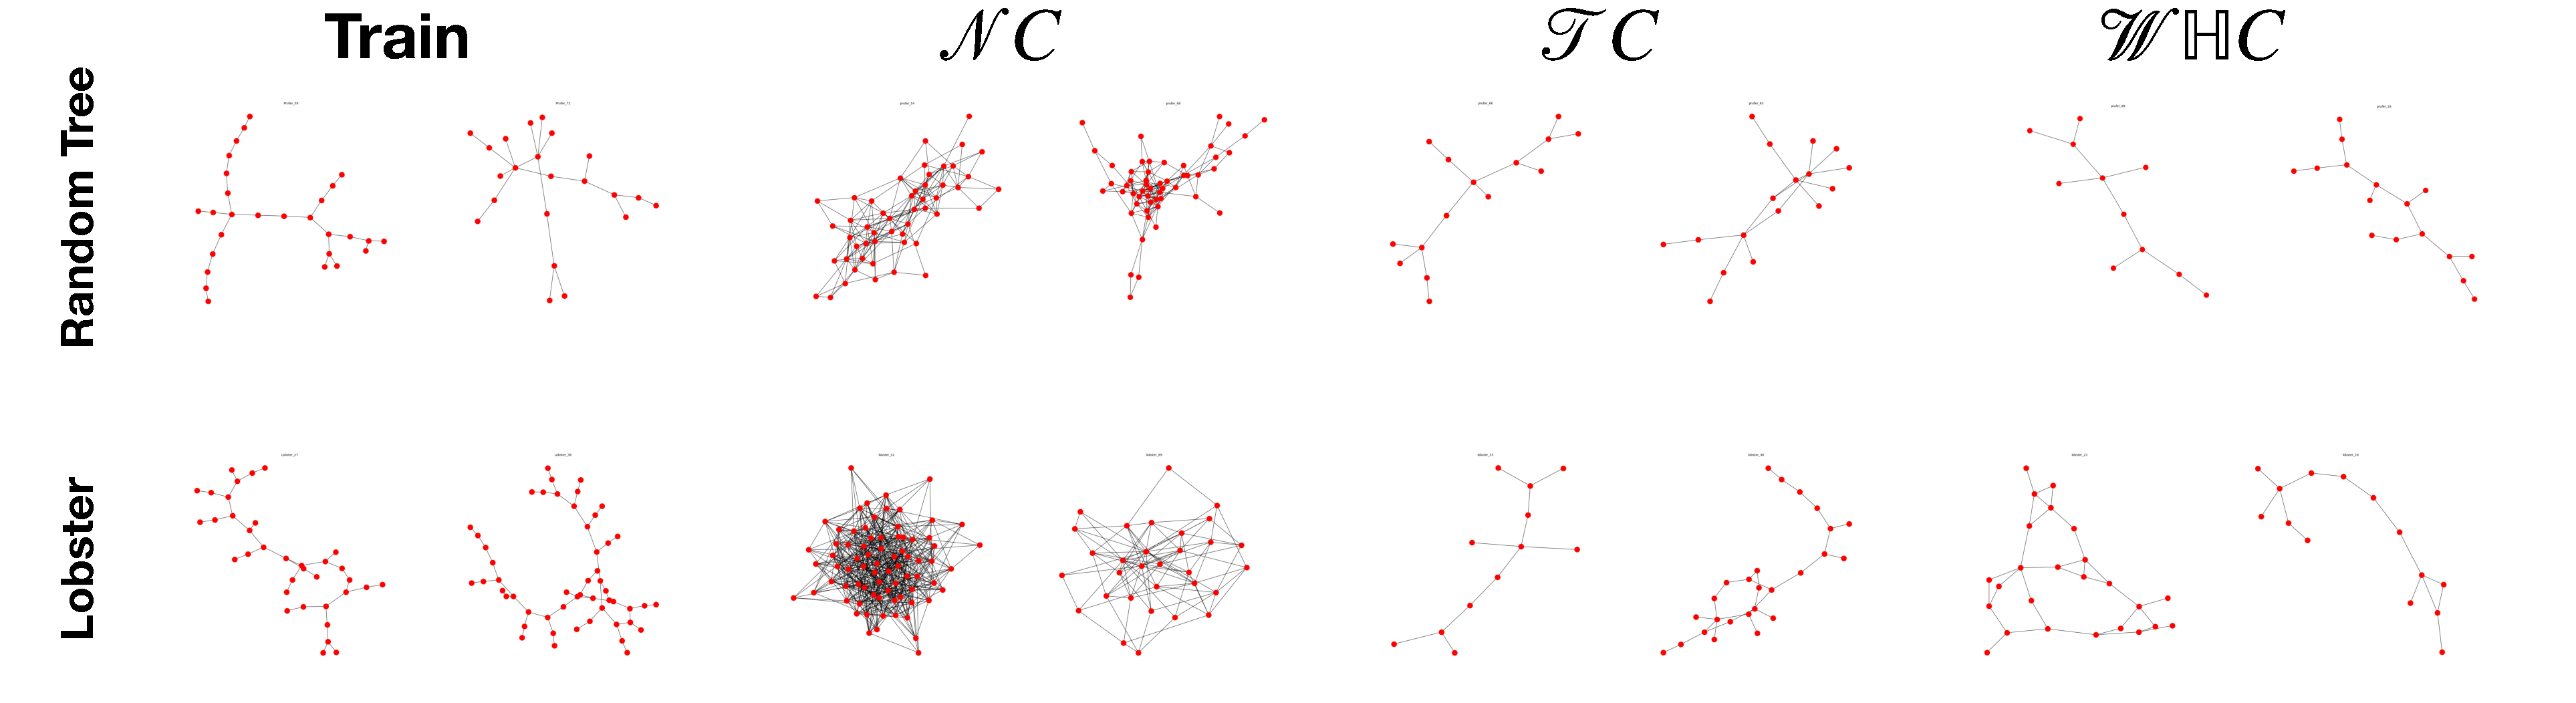
\includegraphics[width=\textwidth]{hyperbolic_graph_gen.pdf}
    \vspace{-5mm}
    \caption{Selected qualitative results on graph generation for lobster and random tree graph.}
    \label{fig:graph_generation_pic}
\end{figure*}

To evaluate the various approaches, we construct $100$ training graphs for each dataset to train our model and then evaluate the quality of the generated graphs. 
Figure 
\cut{
Our evaluation setup closely mirrors that of \cite{liao2019efficient} in that we construct $100$ training graphs with minimum and maximum number of nodes of $20$ and $100$ respectively, and calculate mean maximum discrepancy between distributions of graph statistics for generated and ground truth graphs. In table \ref{graph_gen_table} we present quantitative results for both datasets while Fig. \ref{fig:graph_generation_pic} shows selected generated samples.\cut{and find that both $\mathcal{T}C$ and $\mathcal{W}\mathbb{H}C$ achieve lower MMD scores on all metrics aside from clustering coefficient on Lobster graphs but achieves higher MMD scores on random trees.} As shown in Fig. \ref{fig:graph_generation_pic} generated samples using $\mathcal{N}C$ for the random trees dataset are simply shallow trees with only a handful of nodes which trivially have low MMD scores but do not respect the structure in the data. For lobster graphs, $\mathcal{N}C$ resembles closer to a fully connected graph and is unable to distinguish the hierarchy in the data. These empiricial observations are corroborated in the MMD metrics where we find that both $\mathcal{T}C$ and $\mathcal{W}\mathbb{H}C$ achieve lower MMD scorest. Critically, a significantly higher proportion of generated samples are actually lobster graphs, while none of the samples generated by $\mathcal{N}C$ respect this hierarchical structure.} \cut{Critically, samples generated by the different normalizing flow models demonstrate that flows on hyperbolic spaces are better able to capture the hierarchical structure of data with deeper hierarchies. Critically, a significantly higher proportion of generated samples are actually lobster graphs, while none of the samples generated by $\mathcal{N}C$ respect this hierarchical structure. Fig. \ref{fig:graph_generation_pic} shows selected s}
\cut{
\begin{table*}[]
\label{graph_gen_table}
\begin{scriptsize}
\begin{center}
\begin{tabular}{lllllllllll}
    \toprule
     & \multicolumn{5}{c}{Prufer} &  \multicolumn{5}{c}{Lobster} \\
    
    \midrule
    Model   & Deg. & Clus. & Orb. & Spec. & Acc. & Deg. & Clus. & Orb. & Spec. & Acc.\\
    \midrule
    $\mathcal{N}C$ &$\textbf{0.30}_{\pm0.12}$ & $\textbf{0.59}_{\pm0.40}$& $\textbf{0.57}_{\pm0.38}$& $\textbf{0.31}_{\pm0.15}$ & $\textbf{26.0}_{\pm25.0}$ & $0.47_{\pm3.0\textnormal{e-3}}$ & $1.02_{\pm7.6\textnormal{e-3}}$& $0.28_{\pm0.37}$& $0.50_{\pm0.01}$ & $0.00_{\pm0.0}$  \\
    $\mathcal{T}C$ & $0.31_{\pm0.09}$ & $1.01_{0.29}$& $0.89_{\pm0.11}$& $0.35_{\pm0.09}$ & $5.0_{\pm4.5}$ & $\textbf{0.39}_{\pm0.07}$ & $1.02_{0.62}$& $0.75_{\pm0.38}$& $0.40_{\pm0.11}$ & $\textbf{17.4}_{\pm33.7}$\\
    $\mathcal{W}\mathbb{H}C$ & $0.31_{\pm0.14}$ & $0.72_{\pm0.33}$&  $0.72_{\pm0.33}$& $0.32_{\pm0.14}$ & $16.3_{\pm20.9}$ & $0.41_{\pm0.07}$ & $\textbf{0.96}_{\pm0.43}$& $\textbf{0.47}_{\pm0.44}$& $\textbf{0.39}_{\pm0.13}$ & $11.8_{\pm23.1}$\\
    \bottomrule
\end{tabular}
\end{center}
\caption{Prufer and Lobster.}
\vskip -0.1in
\end{scriptsize}
\end{table*}
}

\begin{table}[]
\label{graph_gen_table}
%\begin{scriptsize}
\begin{center}
\begin{tabular}{llll}
    \toprule
    Model   & Accuracy & Avg. Tri. & Avg. Trans.\\
    \midrule
    $\mathcal{N}C$ & $56.6_{\pm 5.5}$ & $40.9_{\pm 42.7}$ & $0.34_{\pm0.10}$\\
    $\mathcal{T}C$ & $32.1_{\pm 1.9}$ & $98.3_{\pm 89.5}$ & $0.25_{\pm 0.12}$\\
    $\mathcal{W}\mathbb{H}C$ & $\textbf{62.1}_{\pm 10.9}$ & $\textbf{21.1}_{\pm 13.4}$ & $\textbf{0.13}_{\pm0.07}$\\
    \bottomrule
\end{tabular}
\end{center}
\caption{Graph statistics for generation on random trees.}
\vspace{-10pt}
\end{table}

\begin{figure}
    \centering
    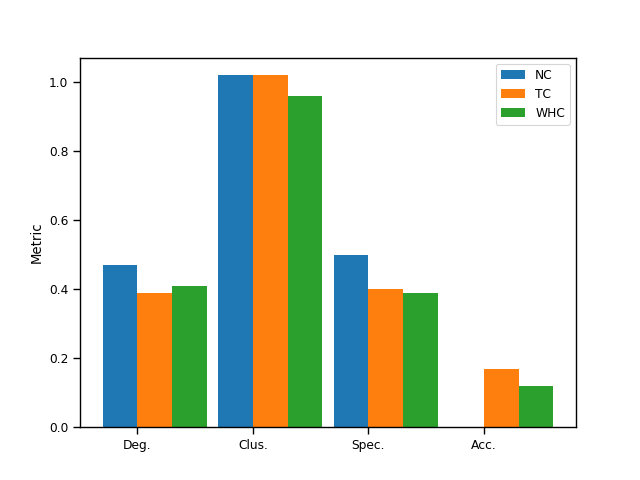
\includegraphics[width=0.9\linewidth]{lobster_graph_gen.png}
    \vspace{-15pt}
    \caption{MMD scores for graph generation on Lobster graphs}
    \label{fig:lobster_graph_gen}
    \vspace{-15pt}
\end{figure}
%cccccccccc

\section{Related Work}
\xhdr{Hyperbolic Geometry in Machine Learning:}
The intersection of hyperbolic geometry and machine learning has recently risen to prominence \cite{dhingra2018embedding,tay2018hyperbolic,law2019lorentzian,khrulkov2019hyperbolic,ovinnikov2019poincar}. Early prior work proposed to embed data into the Poincar\'e ball model \cite{nickel2017poincare,chamberlain2017neural}.
The equivalent Lorentz model was later shown to have better numerical stability properties \cite{nickel2018learning}, and recent work has leveraged even more stable tiling approaches \cite{yu2019numerically}. 
Recent works have extended several conventional deep learning modules (e.g., dense neural network layers and GNN architectures) to hyperbolic space \cite{gulcehre2018hyperbolic,ganea2018hyperbolic, chami2019hyperbolic}.
%To provably bound the numerical error of hyperbolic embeddings in the Lorentz model \cite{yu2019numerically} propose another model of hyperbolic geometry using integer-based tiling. 
%Hyperbolic counterparts to conventional deep learning modules on Euclidean spaces, ---i.e. matrix multiplication, enabled the construction of hyperbolic neural networks (HNNs) \cite{gulcehre2018hyperbolic,ganea2018hyperbolic} and extensions to graph data \cite{liu2019graph,chami2019hyperbolic}.
Latent variable models on hyperbolic space have also been investigated in the context of VAEs, using  generalizations of the normal distribution \cite{nagano2019wrapped,mathieu2019continuous}.\cut{As an extension, \cite{skopek2019mixed} consider a more general case where the latent space of a VAE is a product of Riemannian manifolds with constant and learnable curvatures.} In contrast, our work learns a flexible approximate posterior using a novel normalizing flow designed to use the geometric structure of hyperbolic spaces.
In addition to work on hyperbolic VAEs, there are also several works that explore other non-Euclidean spaces (e.g., spherical VAEs) \cite{davidson2018hyperspherical,falorsi2019reparameterizing,grattarola2019adversarial}.

\xhdr{Normalizing Flows:} 
Normalizing flows (NFs)~\cite{rezende2015variational,dinh2016density} are a class of probabilistic models which use invertible transformations to map samples from a simple base distribution to samples from a more complex learned distribution.\cut{The new density can then be efficiently computed via the change of variable formula making normalizing flow powerful tools for variational inference and generative modeling.}While there are many classes of normalizing flows, see survey \cite{papamakarios2019normalizing,kobyzev2019normalizing}, our work largely follows flows designed with partial ordered dependency as found in affine coupling transformations \cite{dinh2016density}. 
Recently, normalizing flows have also been extended to Riemannian manifolds such as spherical spaces in \citet{gemici2016normalizing}.\cut{The the idea is to (1) map a probability distribution on the Riemannian manifold to its homeomorphic Euclidean space, (2) apply the normalizing flow in this Euclidean space, and (3) map the distribution back to the manifold.} In a different line of work authors in~\citet{wang-wang-2019-riemannian} construct a planar flow  \cite{rezende2015variational} on Riemannian manifolds parameterized by the inverse multiquadratics kernel function. %Relying on affine coupling and GNNs \cite{liu2019graph} develop graph normalizing flows (GNFs) for generating graphs.




\section{Conclusion}
In this paper we introduce two concrete instantiations of normalizing flows on hyperbolic spaces by defining novel coupling transforms. Our first coupling transform, $\mathcal{T}C$, lifts normalizing flow operations by extensively using the tangent space at the origin. We also introduce the $\mathcal{W}\mathbb{H}C$ layer which is specifically designed to explicitly use different regions of the manifold. We further prove that our flows are efficient to sample from, easy to invert and requires only $\mathcal{O}(n)$ cost to compute the change in volume. We demonstrate the effectiveness of constructing normalizing flows for latent variable modelling of hierarchical data where we observe notable gains in structured density estimation compared to Euclidean methods in low dimensions. We further evaluate our approach in graph reconstruction tasks where we see moderate improvements. Lastly, we show generative modelling capabilities of hyperbolic normalizing flows on tree structured data where we observe large qualitative improvements in generated sample quality. 

In terms of limitations and directions for future work, one important limitation is in the numerical error introduced by clamping operations which prevent the creation of deep flow architectures. We hypothesize that this is an inherent limitation of the Lorentz model which maybe alleviated with newer isometries of hyperbolic geometry that use integer-based tiling. While we considered hyperbolic generalizations of the coupling transforms to define our normalizing flows they represent only one class of possible invertible transformations. Designing new classes of invertible transformation like autoregressive and residual flows but for spaces of constant curvature is an interesting direction for future work.

\subsection*{Acknowledgements}
 Funding: AJB is supported by an IVADO Excellence Fellowship. RL was supported by Connaught International Scholarship and RBC Fellowship. WLH is supported by a Canada CIFAR AI Chair. This work was also supported by NSERC Discovery Grants held by WLH and PP. In addition the authors would like to thank Chinwei Huang, Maxime Wabartha, Andre Cianflone and Andrea Madotto for helpful feedback on earlier drafts of this work and Kevin Luk, Laurent Dinh and Niky Kamran for helpful technical discussions. The authors would also like to thank the anonymous reviewers for their comments and feedback and Aaron Lou, Derek Lim, and Leo Huang for catching a bug in the code. 


%\clearpage
\bibliography{bibliography.bib}
\bibliographystyle{icml2020}

\clearpage
\appendix
\onecolumn
\section{Background on Riemannian Geometry}
\label{riemannian_geometry_appendix}
A manifold is a topological space that locally resembles a Euclidean space of the same dimensionality. If $\mathcal{M}$ is an $n-$dimensional manifold then a chart, $\psi: U \to V$, on $\mathcal{M}$ maps an open subset $U$ to an open subset $V \subset \mathbb{R}^n$. Furthermore, the image of the point $p \in U$, denoted $\psi(p) : \mathbb{R}^n$ is termed the local coordinates of $p$ on the chart $\psi$. Examples of manifolds include $\mathbb{R}^n$, the Hypersphere $\mathbb{S}^n$, the Hyperboloid $\mathbb{H}^n$, a torus and so on and so forth. In this paper we take an extrinsic view of the geometry, that is to say a manifold can be thought of as being embedded in a higher dimensional Euclidean space, ---i.e. $\mathcal{M}^n \subset \mathbb{R}^{n+1}$, and inherits the coordinate system of the ambient space. 

\xhdr{Tangent Spaces} Let $p \in \mathcal{M}$ be a point on an $n-$dimensional smooth manifold and let $\gamma(t) \to \mathcal{M}$ be a differentiable parametric curve with parameter $t \in [-\epsilon, \epsilon]$ passing through the point such that $\gamma(0) = p$. Since $\mathcal{M}$ is a smooth manifold we can trace the curve in local coordinates via a chart $\psi$ and the entire curve is given in local coordinates by $x = \psi \circ \gamma(t)$. The tangent vector to this curve at $p$ is then simply $v = (\psi \circ \gamma)'(0)$. Another natural interpretation of the tangent vector of $\gamma$ is by interpreting the point $p$ as a position vector and the tangent vector is then easily interpreted as the velocity vector at that point.\cut{Stated another way the tangent vector is a vector of partial derivatives for every coordinate.} Using this definition the set of all tangent vectors at $p$ is denoted as $\mathcal{T}_p{\mathcal{M}}$, and is called the tangent space at $p$. 

\xhdr{Riemannian Manifold}
A Riemannian metric tensor $g$ on a smooth manifold $\mathcal{M}$ is defined as a family of inner products such that at each point $p \in \mathcal{M}$ the inner product takes vectors from the tangent space at $p$, $g_p= \langle \cdot, \cdot \rangle_p: \mathcal{T}_p\mathcal{M} \times \mathcal{T}_p\mathcal{M} \to \mathbb{R}$. This means $g$ is defined for every point on $\mathcal{M}$ and varies smoothly\footnote{Locally, $g$ can be defined using the basis vectors of the tangent space $g_{ij}(p) = g(\frac{\partial}{\partial p_i}, \frac{\partial}{\partial p_j})$.}. In matrix form the Riemannian metric, $G(p)$, can be expressed as, $\forall u,v \in  \mathcal{T}_p\mathcal{M} \times \mathcal{T}_p\mathcal{M}, \langle u, v \rangle_p = g(p)(u,v) = u^T G(p) v$. A smooth manifold manifold $\mathcal{M}$ which is equipped with a Riemannian metric at every point $p \in \mathcal{M}$ is called a Riemannian manifold. Thus every Riemannian manifold is specified as the tuple $(\mathcal{M},g)$ which define the smooth manifold and its associated Riemannian metric tensor.

Armed with a Riemannian manifold we can now recover some conventional geometric insights such as the length of a parametric curve $\gamma$, the distance between two points on the manifold, local notion of angle, surface area and volume. We define the length of a curve, $L[\gamma] = \int_a^b g_{\gamma (t)} || \gamma '(t)|| dt$. This definition is very similar to the length of a curve on Euclidean spaces if we just observe that the Riemannian metric is $I_n$. Now turning to the distance between points $p$ and $q$ we can reason that it must be the smallest or distance minimizing parametric curve between the points which in the literature are known as \textit{geodesics}. Stated another way: $d(p,q) = \inf \big\{ L[\gamma] \ | \gamma:[a,b] \to \mathcal{M}\big\}$ with ,  $\gamma(a)=p$ and $\gamma(b)=q$. A norm is induced on every tangent space by $g_p$ and is defined as $\mathcal{T}_p\mathcal{M}: || \cdot ||_p :\sqrt{\langle \cdot, \cdot \rangle_p}$. Finally, we can also define an infitisimal volume element on each tangent space and as a result measure $d\mathcal{M}(p) = \sqrt{|G(p)|} dp$, with $dp$ being the Lebesgue measure. 

\section{Background Normalizing Flows}
\label{normalizing_flow_appendix}
Given a parametrized density on $\mathbb{R}^n$ a \textit{normalizing flow} defines a sequence of invertible transformations to a more complex density over the same space via the change of variable formula for probability distributions \cite{rezende2015variational}. Starting from a sample from a base distribution, $z_0 \sim p(z)$, a mapping $f: \mathbb{R}^d \to \mathbb{R}^d$, with parameters $\theta$ that is both invertible and smooth, the log density of $z' = f(z_0)$ is defined as $\log p_{\theta}(z') = \log p(z_0) - \log \det \Big \lvert \frac{\partial f}{\partial z} \Big \rvert$.
\cut{
\begin{align}
    \log p_{\theta}(z') = \log p(z_0) - \log \det \Big \lvert \frac{\partial f}{\partial z} \Big \rvert.
    \label{flow_eqn_1}

\end{align}
}
Where, $p_{\theta}(z')$ is the probability of the transformed sample and $\partial f / \partial x$ is the Jacobian of $f$. To construct arbitrarily complex densities a chain of functions of the same form as $f$ can be defined and through successive application of change of density for each invertible transformation in the flow. Thus the final sample from a flow is then given by $z_k = f_K \circ f_{K-1} ... \circ f_1(z_0)$ and it's corresponding density can be determined simply by $\ln p_{\theta}(z_K) = \ln p(z_0) - \sum_{k=1}^K\ln \det \Big \lvert \frac{\partial f_k}{\partial z_{k-1}} \Big \rvert$. 
Of practical importance when designing normalizing flows is the cost associated with computed the log determinant of the Jacobian which is computationally expensive and can range anywhere from $O(n!)-O(n^3)$ for an arbitrary matrix and a chosen algorithm. However, through an appropriate choice of $f$ this computation cost can be brought down significantly. While there are many different choices for the transformation function, $f$, in this work we consider only RealNVP based flows as presented in \cite{dinh2016density} and \cite{rezende2015variational} due to their simplicity and expressive power in capturing complex data distributions.

\subsection{Variational Inference with Normalizing Flows}
One obvious use case for Normalizing Flows is in learning a more expressive often multi-modal posterior distribution needed in Variational Inference. Recall that a variational approximation is a lower bound to the data log-likelihood. Take for example amortized variational inference in a VAE like setting whereby the posterior $q_{\theta}$ is parameterized and is amenable to gradient based optimization. The overall objective with both encoder and decoder networks:
\begin{align}
    \log p(x) & = \log \int p(x|z)p(z) dz \\
              & \geq \mathbb{E}_{q_{\theta}(z|x)}[\log \frac{p(x,z)}{q_{\theta}(z|x)}] \ \ \ \  (\textnormal{Jensen's Inequality}) \\
              & = \mathbb{E}_{q_{\theta}(z|x)} [\log p(x|z)] + \mathbb{E}_{q_{\theta}(z|x)}\Big[\log \frac{p(z)}{q_{\theta}(z|x)}\Big] \\
              & = \mathbb{E}_{q_{\theta}(z|x)} [\log p(x|z)] - D_{KL}(q_{\theta}(z|x) || p(z)) \label{nn_vae_perspective}
\end{align}
The tightness of the Evidence Lower Bound (ELBO) also known as the negative free energy of the system, $-\mathcal{F}(x)$, is determined by the quality of the posterior approximation to the true posterior. Thus, one way to enrich the posterior approximation is by letting $q_{\theta}$ be a normalizing flow itself and the resultant latent code be the output of the transformation. If we denote $q_0(z_0)$ the probability of the latent code $z_0$ under the base distribution and $z_k$ as the latent code after $K$ flow layers we may rewrite the Free Energy as follows:

\begin{align}
    \mathcal{F}(x) &= \mathbb{E}_{q_{0}(z_0)}[\log q_k(z_k) - \log p(x,z_k)] \\
    &= \mathbb{E}_{q_{0}(z_0)}\Big[\log q_0(z_0) - \sum_{k=1}^K\ln \det \Big \lvert \frac{\partial f_k}{\partial z_{k-1}} \Big \rvert - \log p(x,z_k)\Big]\\
    &= D_{KL}(q_0(z_0)|| p(z_k)) - \mathbb{E}_{q_{0}(z_0)}\Big[\sum_{k=1}^K\ln \det \Big \lvert \frac{\partial f_k}{\partial z_{k-1}} \Big \rvert - \log p(x|z_k)\Big]
\end{align}
For convenience we may take $q_0 = \mathcal{N}(\mu, \sigma^2)$ which is a reparametrized gaussian density and $p(z) = \mathcal{N}(0, I)$ a standard normal. 

\subsection{Euclidean RealNVP}
\label{Euclidean_RealNVP_appendix}
Computing the Jacobian of functions with high-dimensional domain and codomain and computing the determinants of large matrices are in general computationally very expensive. Further complications can arise with the restriction to bijective functions make for difficult modelling of arbitrary distributions. A simple way to significantly reduce the computational burden is to design transformations such that the Jacobian matrix is triangular resulting in a determinant which is simply the product of the diagonal elements. In \cite{dinh2016density}, real valued non-volume preserving (RealNVP) transformations are introduced as simple bijections that can be stacked but yet retain the property of having the composition of transformations having a triangular determinant. To achieve this each bijection updates a part of the input vector using a function that is simple to invert,
but which depends on the remainder of the input vector in a complex way. Such transformations are denoted  as affine coupling layers. Formally, given a $D$ dimensional input $x$ and $d < D$, the output $y$ of an affine coupling layer follows the equations:
\begin{align}
    y_{1:d} & = x_{1:d} \\
    y_{d+1:D} & = x_{d+1:D} \odot \textnormal{exp}(s(x_{1:d})) + t(x_{1:d}).
\end{align}
Where, $s$ and $t$ are parameterized scale and translation functions. As the second part of the input depends on the first, it is easy to see that the Jacobian given by this transformation is lower triangular. Similarly, the inverse of this transformation is given by:
\begin{align}
     x_{1:d} & = y_{1:d} \\
    x_{d+1:D} & = (y_{d+1:D} - t(y_{1:d})\odot \textnormal{exp}(-s(y_{1:d})).
\end{align}
Note that the form of the inverse does not depend on calculating the inverses of either $s$ or $t$ allowing them to be complex functions themselves. Further note that with this simple bijection part of the input vector is never touched which can limit the expressiveness of the model. A simple remedy to this is to simply reverse the elements that undergo scale and translation transformations prior to the next coupling layer. Such an alternating pattern ensures that each dimension of the input vector depends in a complex way given a stack of couplings allowing for more expressive models. Finally, the Jacbobian of this transformation is a lower triangular matrix,
\begin{equation} 
    \frac{\partial y}{\partial x} = \begin{bmatrix}
                                    \mathbb{I}_{d} & 0 \\
                                
                                   \frac{\partial y_{d+1:D}}{x^T_{1:d}} & \textnormal{diag}(\textnormal{exp}s(x_{1:d}))
                                    \end{bmatrix}.
\end{equation}

\section{Change of Variable for Tangent Coupling}
\label{tangent_coupling_proof_appendix}
\begin{equation}
    \textbf{y} =  \textnormal{exp}_{\textbf{o}}(b \odot \tilde{x} + (1 - b)\odot(\tilde{x} \odot \sigma(s(b \odot \tilde{x})) + t(b \odot \tilde{x}))),
\end{equation}
where $\tilde{x} = \log_{\textbf{o}}(x)$ is a point on the tangent space at $\textbf{o}$. Similar to the Euclidean RealNVP, we wish to calculate the jacobian determinant of this overall transformation. We do so by first observing that the overall transformation is a valid composition of functions: $y := \textnormal{exp}_{\textbf{o}} \circ f\circ \log_{\textbf{o}}(\textbf{x})$, where $z = f(\tilde{x})$ is the flow in tangent space. Utilizing the chain rule and the identity that the determinant of a product is the product of the determinants of its constituents we may decompose the jacobian determinant as,

\begin{equation}
    \textnormal{det}\Big (\frac{\partial \textbf{y}}{\partial \textbf{x}}\Big) =  \textnormal{det}\Big (\frac{\partial \textnormal{exp}_{\textbf{o}}(z)}{\partial z}\Big) \cdot \textnormal{det}\Big (\frac{\partial f(\tilde{x})}{\partial \tilde{x}}\Big) \cdot  \textnormal{det}\Big (\frac{\partial \log_{\textbf{o}}(\textbf{x})}{\partial \textbf{x}}\Big)
    \label{jac_det_tangent_flow_1}.
\end{equation}
Tackling each term on RHS of Eq. \ref{jac_det_tangent_flow_1} individually, $ \textnormal{det}\Big (\frac{\partial \textnormal{exp}_{\textbf{o}}(z)}{\partial z}\Big) = \Big(\frac{\sinh(||z||_{\mathcal{L}})}{||z||_{\mathcal{L}}}\Big)^{D-1}$ as derived in \cite{nagano2019wrapped}. As the logarithmic map is the inverse of the exponential map the jacobian determinant is also the inverse ---i.e.  $\textnormal{det}\Big (\frac{\partial \log_{\textbf{o}}(\textbf{x})}{\partial \textbf{x}}\Big) = \Big(\frac{\sinh(||\log_{\textbf{o}}(\textbf{x})||_{\mathcal{L}})}{||\log_{\textbf{o}}(\textbf{x})||_{\mathcal{L}}}\Big)^{1-D}$. For the middle term in Eq. \ref{jac_det_tangent_flow_1} we proceed by selecting the standard basis $\{e_1, e_2, ... e_n\}$ which is an orthonormal basis  with respect to the Lorentz inner product. Without loss of generality define $b_k = 1$ if $0 \leq k \leq d$ and $b_k = 0$ for $d < k \leq D$. The directional derivative with respect to a basis element $e_k$ is computed as follows:

\begin{align*}
    \textnormal{d}f(\tilde{x}) &= \frac{\partial}{\partial \epsilon} \Big |_{\epsilon=0} f(\tilde{x} + \epsilon e_k)\\
    & = \frac{\partial}{\partial \epsilon} \Big |_{\epsilon=0} \{b \odot (\tilde{x} + \epsilon e_k) + (1 - b)\odot((\tilde{x} + \epsilon e_k) \odot \sigma(s(b \odot (\tilde{x} + \epsilon e_k))) + t(b \odot (\tilde{x} + \epsilon e_k)))\} \\
    &= b \odot  e_k + \frac{\partial}{\partial \epsilon} \Big |_{\epsilon=0}\{ (1 - b)\odot((\tilde{x} + \epsilon e_k) \odot \sigma(s(b \odot (\tilde{x} + \epsilon e_k))) + t(b \odot (\tilde{x} + \epsilon e_k)))\} \\
\end{align*}
As $b \in [0,1]^D$ is a binary mask, it is easy to see that if $b_k =1$ then only the first term on the RHS remains and the directional derivative with respect to $e_k$ is simply the basis vector itself. Conversely, if $b_k =0$ then the first term goes to zero and we are left with the second term,

\begin{align*}
    \textnormal{d}f(\tilde{x}) &= \frac{\partial}{\partial \epsilon} \Big |_{\epsilon=0}\{ (1 - b)\odot((\tilde{x} + \epsilon e_k) \odot \sigma(s(b \odot (\tilde{x} + \epsilon e_k))) + t(b \odot (\tilde{x} + \epsilon e_k)))\} \\
    &=  \frac{\partial}{\partial \epsilon} \Big |_{\epsilon=0}\{ (1 - b)\odot((\tilde{x} + \epsilon e_k) \odot \sigma(s(b \odot \tilde{x})) + t(b \odot \tilde{x}))\} \\
    &= e_k \odot \sigma(s(b \odot \tilde{x})).
\end{align*}
Where in the second line we've used the fact $b \odot \epsilon e_k = 0$. All together, the directional derivatives computed using our chosen basis elements are,

\begin{equation*}
    \textnormal{d}f(\tilde{x}) = (e_1, e_2, \dots e_d, e_{d+1}\odot \sigma(s(b \odot \tilde{x})), \dots e_{D}\odot \sigma(s(b \odot \tilde{x}))).
\end{equation*}
The volume factor given by this linear map is $\textnormal{det}( \textnormal{d}f(\tilde{x})) = \sqrt{G^TG}$, where $G$ is the matrix of all directional derivatives. As the basis elements are orthogonal all non-diagonal entries of $G^TG$ go to zero and the determinant is the product of the Lorentz norms of each component. As $||e_k||_{\mathcal{L}} =1$ and $||e_{k}\odot \sigma(s(b \odot \tilde{x}))||_{\mathcal{L}} = ||e_{k}\odot \sigma(s(b \odot \tilde{x}))||_2$ for $\mathcal{T}_{\mathbf{o}}H^{D,1}$ the overall determinant is then $\textnormal{d}f(\tilde{x}) = \textnormal{diag} \ \sigma(s(b \odot \tilde{x}))$. Finally, the full log jacobian determinant of Tangent RealNVP is given by,

\begin{equation}
    \log \textnormal{det}\Big (\frac{\partial \textbf{y}}{\partial \textbf{x}}\Big) = \Big(\frac{\sinh(||z||_{\mathcal{L}})}{||z||_{\mathcal{L}}}\Big)^{D-1} + \textnormal{diag} \ \sigma(s(b \odot \tilde{x})) + \Big(\frac{\sinh(||\log_{\textbf{o}}(\textbf{x})||_{\mathcal{L}})}{||\log_{\textbf{o}}(\textbf{x})||_{\mathcal{L}}}\Big)^{1-D}
\end{equation}

Thus the overall computational cost is only slightly larger than the regular Euclidean RealNVP, $\mathcal{O}(kD)$, where $k$ is a constant.

\section{Change of Variable for Wrapped Hyperbolic Coupling}
\label{wrapped_coupling_proof_appendix}
We consider the following function $f : \mathbb{H}^n \rightarrow \mathbb{H}^n$, which we use to define a normalizing flow in $n$-dimensional hyperbolic space (represented via the hyperboloid/Lorentz model): 
\begin{equation}\label{eq:mainflow}
    f(\mb{x}) = \textnormal{exp}_{\textbf{o}}\left( b \odot \tilde{
    \mb{x}} + (1-b) \odot \log_{\textbf{o}}\Big( \textnormal{exp}_{t(b \odot \tilde{\mb{x}})}\big(\textnormal{PT}_{\textbf{o}\to t(b \odot \tilde{\mb{x}}) }((1-b) \odot \tilde{\mb{x}} \odot \sigma(s(b \odot \tildex)))\big)\Big) \right),
\end{equation}

where $\tildex = \log_\mb{o}(\mb{x}) \in \mc{T}_\mb{o}\mbb{H}^n$ is the projection of $\mb{x} \in \mbb{H}^n$ to the tangent space at the origin, i.e, $\mc{T}_\mb{o}\mbb{H}^n$. 
The $b$ term is assumed to be a binary mask and without loss of generality we define $b$ so that
$$ 
b_i = 
\begin{cases}
1 &\textrm{if $i\leq d$}\\
0 &\textrm{otherwise},
\end{cases}
$$
where $0 < d < n$.
In Equation \eqref{eq:mainflow} the function $s : \mc{T}_o\mbb{H}^n \rightarrow \mc{T}_o\mbb{H}^n$ is an arbitrary function on the tangent space at the origin and $\sigma$ denotes the logistic function.
The function $t : \mc{T}_o\mbb{H}^n \rightarrow \mbb{H}^* \subset {H}^n$ is a map from the tangent space at the origin to a subset of hyperbolic space defined by the set of points satisfying the condition that $\mb{v}_i = 0, \forall i=2...d, v_i \in \mbb{H}^n$ (under their representation in the Lorentz model).

Our goal is to derive the Jacobian determinant of $f$, i.e., 
\begin{equation}
    \left|\textrm{det}\left(\frac{\partial f(\mb{x})}{\partial \mb{x}}\right)\right|,
\end{equation}
where $\frac{\partial f(\mb{x})}{\partial \mb{x}} : \mc{T}_\mb{x}\mbb{H}^n \rightarrow \mc{T}_{f(\mb{x})}\mbb{H}^n$ is Jacobian of $f$.
To do so, we will use the following facts without proof or justification:
\begin{itemize}
    \item 
    \textbf{Fact 1: }The chain rule for determinants, i.e., the fact that
    \begin{equation}
        \left|\textrm{det}\left(\frac{\partial f(\mb{x})}{\partial \mb{x}}\right)\right| =  \left|\textrm{det}\left(\frac{\partial f(\mb{x})}{\partial \mb{v}}\right)\right| \left|\textrm{det}\left(\frac{\partial \mb{v}}{\partial \mb{x}}\right)\right|,
    \end{equation}
    where $\mb{v}$ is introduced via a valid change of variables. 
    \item 
    \textbf{Fact 2: } The Jacobian determinant for the exponential map $\exp_\mb{u}(\mb{v}) = \mc{T}_{u}\mbb{H}^n \rightarrow \mbb{H}^n$ is given by
    \begin{equation}
        \left|\textrm{det}(\exp_\mb{u}(\mb{v}))\right| = \left(\frac{\sinh(\|\mb{v}\|_\mc{L})}{\|\mb{v}\|_\mc{L}}\right)^{n-1}.
    \end{equation}
        \item 
    \textbf{Fact 3: } The Jacobian determinant for the logarithmic map $\log_\mb{u}(\mb{v}) = \mbb{H}^n \rightarrow \mc{T}_u\mbb{H}^n$ is given by
    \begin{equation}
        \left|\textrm{det}(\log_\mb{u}(\mb{v})\right| = \left(\frac{\sinh(\|\log_\mb{u}(\mb{v})\|_\mc{L})}{\|\log_\mb{u}(\mb{v})\|_\mc{L}}\right)^{1-n}.
    \end{equation}
    \item
     \textbf{Fact 4: } The Jacobian determinant for parallel transport $\textnormal{PT}_{\mb{u} \rightarrow \mb{t}}(\mb{v}) = \mc{T}_\mb{u}\mbb{H}^n \rightarrow \mc{T}_t\mbb{H}^n$ is given by
    \begin{equation}
        \left|\textrm{det}\left(\textnormal{PT}_{\mb{u} \rightarrow \mb{t}}(\mb{v})\right)\right| = 1.
    \end{equation}
\end{itemize}
Fact 2 and Fact 4 are proven in Nagano et al (2019)'s ``A Wrapped Normal Distribution on Hyperbolic Space for Gradient-Based Learning'' and Fact 3 follows from the fact that the determinant of the inverse of a function is the inverse of that function's determinant. 
We will use similar arguments to obtain our determinant as were used in Nagano et al, and we refer the reader to Appendix A.3 in their work for background. 

Our main claim is as follows
\begin{prop}
The Jacobian determinant of the function $f$ in Equation \eqref{eq:mainflow} is:
\begin{align*}
  \left|\textnormal{det}\left(\frac{\partial f(\mb{x})}{\partial \mb{x}}\right)\right| &= \Big(\frac{\sinh(||\mb{z}||_{\mathcal{L}})}{||\mb{z}||_{\mathcal{L}}}\Big)^{n-1} \times \Big(\frac{\sinh(||\mb{q}||_{\mathcal{L}})}{||\mb{q}||_{\mathcal{L}}}\Big)^{n-d-1} \times  \prod_{i=d+1}^n\sigma(s(b \odot \tilde{x}))_i \ \times \\
    & \quad \Big(\frac{\sinh(||\log_{\textbf{o}}(\mb{q})||_{\mathcal{L}})}{||\log_{\textbf{o}}(\mb{q})||_{\mathcal{L}}}\Big)^{d+1-n} \times \Big(\frac{\sinh(||\log_{\textbf{o}}(\textbf{x})||_{\mathcal{L}})}{||\log_{\textbf{o}}(\textbf{x})||_{\mathcal{L}}}\Big)^{1-n},
\end{align*}
where 
$$
\mb{z} =  b \odot \tilde{
    \mb{x}} + \log_{\textbf{o}}\Big( \textnormal{exp}_{t(b \odot \tilde{\mb{x}})}\big(\textnormal{PT}_{\textbf{o}\to t(b \odot \tilde{\mb{x}}) }((1-b) \odot \tilde{\mb{x}} \odot \sigma(s(b \odot \tildex)))\big)\Big)
$$
and
$$
 \mb{q} = \textnormal{PT}_{\textbf{o}\to t(b \odot \tilde{\mb{x}}) }((1-b) \odot \tilde{\mb{x}} \odot \sigma(s(b \odot \tildex))).
$$
\end{prop}
\begin{proof}
We first note that 
\begin{equation}
\left|\textnormal{det}\left(\frac{\partial f(\mb{x})}{\partial \mb{x}}\right)\right| = \left|\textrm{det}\left(\frac{\partial f(\mb{x})}{\partial \mb{z}}\right)\right| \times \left|\textrm{det}\left(\frac{\partial \mb{z}}{\partial \tildex}\right)\right| \times \left|\textrm{det}\left(\frac{\partial \tildex}{\partial \mb{x}}\right)\right| 
\end{equation}
by the chain rule (recalling that $\tildex = \log_\mb{o}(\mb{x})$).
Now, we have that 
\begin{equation}
\left|\textrm{det}\left(\frac{\partial f(\mb{x})}{\partial \mb{z}}\right)\right| = \Big(\frac{\sinh(||\mb{z}||_{\mathcal{L}})}{||\mb{z}||_{\mathcal{L}}}\Big)^{n-1}
\end{equation}
by Fact 2.
And, 
\begin{equation}
\left|\textrm{det}\left(\frac{\partial \tildex}{\partial \mb{x}}\right)\right| = \Big(\frac{\sinh(||\log_{\textbf{o}}(\textbf{x})||_{\mathcal{L}})}{||\log_{\textbf{o}}(\textbf{x})||_{\mathcal{L}}}\Big)^{1-n}
\end{equation}
by Fact 3.
Thus, we are left with the term
$$
\left|\textrm{det}\left(\frac{\partial \mb{z}}{\partial \tildex}\right)\right|.
$$
To evaluate this term, we rely on the following Lemma:

\begin{lemma}
Let $g : \mc{T}_\mb{o}\mbb{H}^n \rightarrow \mc{T}_\mb{o}\mbb{H}^n$ be a function from the tangent space at the origin to the tangent space at the origin defined as:
\begin{equation}\label{eq:g}
g(\tildex) = \mb{z} = b \odot \tilde{
    \mb{x}} + \log_{\textbf{o}}\Big( \textnormal{exp}_{t(b \odot \tilde{\mb{x}})}\big(\textnormal{PT}_{\textbf{o}\to t(b \odot \tilde{\mb{x}}) }((1-b) \odot \tilde{\mb{x}} \odot \sigma(s(b \odot \tildex)))\big)\Big).
\end{equation}
Now, define a function $g^* : \mc{T}_\mb{o}\mbb{H}^{n-d} \rightarrow \mc{T}_\mb{o}\mbb{H}^{n-d}$ which acts on the subspace of $\mc{T}_\mb{o}\mbb{H}^{n-d}$ corresponding to the standard basis elements $\mb{e}_{d+1}, ..., \mb{e}_n$ as
\begin{equation}\label{eq:gstar}
g^*(\tildex_{d+1:n}) =   \log_{\mb{o}_{d+1:n}}\Big( \textnormal{exp}_{\mb{t}_{d+1:n}}\big(\textnormal{PT}_{\mb{o}_{d+1:n} \to \mb{t}_{d+1:n}}( \tilde{\mb{x}}_{d+1:n} \odot \sigma(\mb{s}))\big)\Big),
\end{equation}
where $\tildex_{d+1:n}$ denotes the portion of the vector $\tildex$ corresponding to the standard basis elements $\mb{e}_{d+1}, ..., \mb{e}_n$ and $\mb{s}$ and $\mb{t}$ are constants (which depend on $\tildex_{2:d}$).
In Equation \eqref{eq:gstar}, we use $\mb{o}_{d+1:n} \in \mbb{H}^{n-d}$ to denote the vector corresponding to only the dimensions $d+1, ..., n$ and similarily for $\mb{t}_{d+1:n}$.
Then we have that
\begin{equation}
    \left|\textnormal{det}\left(\frac{\partial \mb{z}}{\partial \tildex}\right)\right| =    \left|\textnormal{det}\left(\frac{\partial g^*(\tildex_{d+1:n})}{\partial \tildex_{d+1:n})}\right)\right|.
\end{equation}
\end{lemma}
\begin{proof}
First note that by design we have that 
\begin{equation}
    [0,0..,0] \oplus g^*(\tildex_{d+1:n}) = \log_{\textbf{o}}\Big( \textnormal{exp}_{t(b \odot \tilde{\mb{x}})}\big(\textnormal{PT}_{\textbf{o}\to t(b \odot \tilde{\mb{x}}) }((1-b) \odot \tilde{\mb{x}} \odot \sigma(s(b \odot \tildex)))\big)\Big),
\end{equation}
i.e., the output of $g^*$ is equal to right hand side of Equation \eqref{eq:g} after prepending/concatenating 0s to the output of $g^*$. 

Now, we can evaluate 
$$
\left|\textrm{det}\left(\frac{\partial \mb{z}}{\partial \tildex}\right)\right|
$$
by examining the directional derivative with respect to a set of basis elements of $\mc{T}_\mb{o}\mbb{H}^{n}$.
Now, given that this is the tangent space at the origin, we know that the standard (i.e., Euclidean) basis elements $\mb{e}_2, ..., \mb{e}_n$ form a valid basis for this subspace, since they are orthogonal under the Lorentz normal and orthogonal to the origin itself. 
Now, we can note first that
\begin{equation}
    D_{\mb{e}_i}g(\tildex) = \mb{e}_i, \forall i=2...d.
\end{equation}
In other words, the directional derivative for the first $d$ basis elements is the simply the basis elements themselves. This can be verified by taking the definition of the directional derivative:
\begin{equation}
     D_{\mb{e}_i}g(\tildex)  = \frac{\partial}{\partial \epsilon}\Big|_{\epsilon = 0}g(\tildex + \epsilon\mb{e}_i)
\end{equation}
and noting that the 
$$
\log_{\textbf{o}}\Big( \textnormal{exp}_{t(b \odot \tilde{\mb{x}})}\big(\textnormal{PT}_{\textbf{o}\to t(b \odot \tilde{\mb{x}}) }((1-b) \odot \tilde{\mb{x}} \odot \sigma(s(b \odot \tildex)))\big)\Big)
$$
term must equal zero since $(1-b)\odot \mb{e}_i = \mb{0}, \forall i = 2, ..., d$ by design. 
Now, for the basis elements $\mb{e}_i$ with $i>d$ we have that
\begin{equation}
     D_{\mb{e}_i}g(\tildex) \perp \mb{e}_j, \forall i=d+1, ..., n, j=2...,d.
\end{equation}
This holds because 
\begin{align}
D_{\mb{e}_i}g(\tildex)  &= \frac{\partial}{\partial \epsilon}\Big|_{\epsilon = 0}g(\tildex + \epsilon\mb{e}_i) \\
 &= \frac{\partial}{\partial \epsilon}\Big|_{\epsilon = 0}    \log_{\textbf{o}}\Big( \textnormal{exp}_{t(b \odot \tilde{\mb{x}})}\big(\textnormal{PT}_{\textbf{o}\to t(b \odot \tilde{\mb{x}}) }((1-b) \odot \tilde{\mb{x}} \odot \sigma(s(b \odot \tildex)))\big)\Big) 
\end{align}
since $b \odot \mb{e}_i = \mb{0}, \forall i = d+1, ..., n$ by design and because
\begin{equation}
   \log_{\textbf{o}}\Big( \textnormal{exp}_{t(b \odot \tilde{\mb{x}})}\big(\textnormal{PT}_{\textbf{o}\to t(b \odot \tilde{\mb{x}}) }((1-b) \odot \tilde{\mb{x}} \odot \sigma(s(b \odot \tildex)))\big)\Big) \perp \mb{e}_j, \forall \tildex \in \mc{T}_\mb{o}\mbb{H}^n, \forall  j=2...,d.
\end{equation}
due to the $(1-b)$ term inside the parallel transport and by our design of the function $t$. 
Together, these facts give that the Jacobian matrix for $g$ (under the basis $\mb{e}_2, ..., \mb{e}_n$) has the following block form:
\begin{equation}
   \left(\frac{\partial \mb{z}}{\partial \tildex}\right) = \left[\begin{BMAT}{cc}{cc}
    \mb{I} & \mb{0} \\
    \mb{A} & \frac{\partial g^*(\tildex_{d+1:n})}{\partial \tildex_{d+1:n})}
    \end{BMAT}\right]
\end{equation}
and by the properties of determinants of block matrices we have that
\begin{equation}
    \left|\textnormal{det}\left(\frac{\partial \mb{z}}{\partial \tildex}\right)\right| =    \left|\textnormal{det}\left(\frac{\partial g^*(\tildex_{d+1:n})}{\partial \tildex_{d+1:n})}\right)\right|
\end{equation}
\end{proof}
Given Lemma 1, all that remains is to evaluate 
\begin{equation}
    \left|\textnormal{det}\left(\frac{\partial g^*(\tildex_{d+1:n})}{\partial \tildex_{d+1:n})}\right)\right|.
\end{equation}
This can again be done by the chain rule, where we use Facts 2-4 to compute the determinant for exponential map, logarithmic map, and parallel transport.
Finally, the Jacobian determinant for the term
\begin{equation}
    \tildex \odot \sigma(s(b \odot \tildex)))
\end{equation}
can easily be computed as $\prod_{i=d+1}^n\sigma(s(b \odot \tilde{x}))_i$ since the standard Euclidean basis is a basis for the tangent space at the origin.
(These full derivations will be added at a later time.)
\end{proof}

\cut{

\section{Decoders}
\noindent
\textbf{Issue:} Our VGAE models are trained using a cross-entropy loss over the predictions
\begin{equation}
    \hat{P}(A[i,j] = 1 | \Theta),
\end{equation}
where $\Theta$ is our encoder/decoder model parameters. However, many of our decoders are not giving proper probabilities, 
for example taking a sigmoid of distances between node latents
\begin{equation}
    \hat{P}(A[i,j] = 1 | \Theta) = \sigma(-d(\mb{z}_i, \mb{z}_j))
\end{equation}
is improper since $\sigma(-d(\mb{z}_i, \mb{z}_j)) \in [0,0.5]$ and is not surjective onto $[0,1]$. (The root cause is the fact that $d(\mb{z}_i, \mb{z}_j) \geq 0$.)
{\bf Note that this is an issue at both training and inference, as our cross-entropy loss during training will also struggle to learn when using improper probability inputs.}


Note that the dot-product decoder does not have this problem because 
\begin{equation}
  \hat{P}(A[i,j] = 1 | \Theta) = \sigma(\mb{z}_i^\top \mb{z}_j) 
\end{equation}
is surjective on $[0,1]$ since $\mb{z}_i^\top \mb{z}_j\in [-\inf, \inf]$.
{\bf However, we want to use a distance-based decoder, because that allows us to leverage the structure of the hyperbolic space in the most proper/elegant/intuitive way.}\\

\noindent
\textbf{Direct Solution} We use a well-defined softmax. The most direct solution to give proper probabilties for edges within a single graph based on distances would be:
\begin{equation}
    \hat{P}(A[i,j] = 1 | \Theta) = \sigma(p)\times\frac{\exp(d(\mb{z}_i, \mb{z}_j))}{\sum_{k=1}^{n}\sum_{l=l+1}^{n}\exp(d(\mb{z}_k, \mb{z}_l))} 
\end{equation}
where $p \in \mathbb{R}$ is a learnable parameter that controls the density of the graph.  
Note that here we are normalizing over all possible edges in the graph. 
Thus, a pair of nodes that are close together {\em relative to the average pair of nodes in the graph}, will tend to be connected. 
The $\sigma(p)$ term controls the density of the graph. 
{\bf This equation would be perfect if we were only learning a model over a single graph... However, if we are training over a distribution of multiple graphs that might have different numbers of nodes then the probabilities will all be lower in larger graphs, which is no good.}
In particular, if all the nodes are equidistant then we will get lower probabilities for a graph with more nodes...
A natural way to fix this is as follows:
\begin{equation}
    \hat{P}^{\textrm{fixed}}(A[i,j] = 1 | \Theta) = \sigma(p)\times\frac{\exp(d(\mb{z}_i, \mb{z}_j))}{\sum_{k=1}^{n}\sum_{l=l+1}^{n}\exp(d(\mb{z}_k, \mb{z}_l))} \times \left(\max_{i',j'}\left\{\frac{\exp(d(\mb{z}_{i'}, \mb{z}_{j'}))}{\sum_{k=1}^{n}\sum_{l=l+1}^{n}\exp(d(\mb{z}_k, \mb{z}_l))}\right\}\right)^{-1}
\end{equation}
That is, we normalize the softmax score by the inverse of the maximum softmax value for a graph.
This ensures that the decoder simplifies to the Erdos-Renyi model (with edge probability $\sigma(p)$) when all pairwise distances are equal (in expectation), regardless of how many nodes are in the graph.
Note that the $\sigma(p)$ term is important since it is what allows the model to learn the density of the graph. 



}

\section{Model Architectures and Hyperparameters}
\label{model_arch_and_hyperparams}
\end{document}


% This document was modified from the file originally made available by
% Pat Langley and Andrea Danyluk for ICML-2K. This version was created
% by Iain Murray in 2018, and modified by Alexandre Bouchard in
% 2019 and 2020. Previous contributors include Dan Roy, Lise Getoor and Tobias
% Scheffer, which was slightly modified from the 2010 version by
% Thorsten Joachims & Johannes Fuernkranz, slightly modified from the
% 2009 version by Kiri Wagstaff and Sam Roweis's 2008 version, which is
% slightly modified from Prasad Tadepalli's 2007 version which is a
% lightly changed version of the previous year's version by Andrew
% Moore, which was in turn edited from those of Kristian Kersting and
% Codrina Lauth. Alex Smola contributed to the algorithmic style files.
